\section{Experiments}\label{sec:exp}


\subsection{Datasets and baselines}

To show the effectiveness of the proposed method, I use MERL \cite{Matusik2003jul} and RGL (51 isotropic materials) \cite{dupuy2018adaptive} datasets, which are the most commonly used BRDF datasets that include isotropic materials. The MERL dataset \cite{Matusik2003jul} consists of 100 real-world materials, covering a wide range of appearances. Each material includes reflectance measurements from a dense set of directions, parameterized as the spherical angles ($\theta$, $\phi$) of the $H$ and $D$ vectors from the Rusinkiewicz parameterization \cite{rusinkiewicz1998new}. Each colour channel has a resolution of 90 × 90 × 180, leading to $1\,458\,000$ reflectance measurements. 



\subsection{Sparse BRDF reconstruction}\label{sec:brdf_rec}

To understand the reconstruction capacity of HyperBRDF, I first train the model with all available samples ($1\,458\,000$). I observe that reducing the number of samples by around half ($640\,000$) results in a similar performance (see Table \ref{table: ours_large_samples}). For comparison with baselines, I train the hypernetwork model with 80 MERL materials that are randomly selected. I leave the remaining 20 materials for testing. I also train HyperBRDF with a mixed dataset of 80 MERL materials and 51 isotropic RGL materials. I later test the trained model on the same test dataset (20 MERL materials). I apply a separate log relative mapping to RGL materials by computing the median over the isotropic RGL dataset.
 
I qualitatively compare the results against the ground truths through renderings of the materials. The renderings are obtained by a Mitsuba renderer with an environment map illumination. HyperBRDF can capture the diffuse colours of varying unseen appearances even for the materials with specular components. 


The main advantage of the hypernetwork architecture is that it is flexible in the number of samples fed to the network. That is, we can reconstruct unseen materials with fewer samples than the sample number used during training. Thanks to its built-in nonlinear interpolation that comes from the hyponet, I obtain high quality reconstruction results with fewer samples. 

Considering the hypernetwork architecture, I understand that the gap between reconstruction results with sparse samples relies on the embeddings $z$ (latent vectors). I hence analyse the embeddings for the materials reconstructed with varying number of samples. Figure \ref{fig:tsne-vis-imputation} illustrates the t-SNE clustering of the test embeddings with different number of samples. It is visible that the embeddings of the same material reconstructed with different sample sizes lie close in the t-SNE space.

\begin{figure}[t]
  \centering
  % \fbox{\rule{0pt}{2in} \rule{0.9\linewidth}{0pt}}
   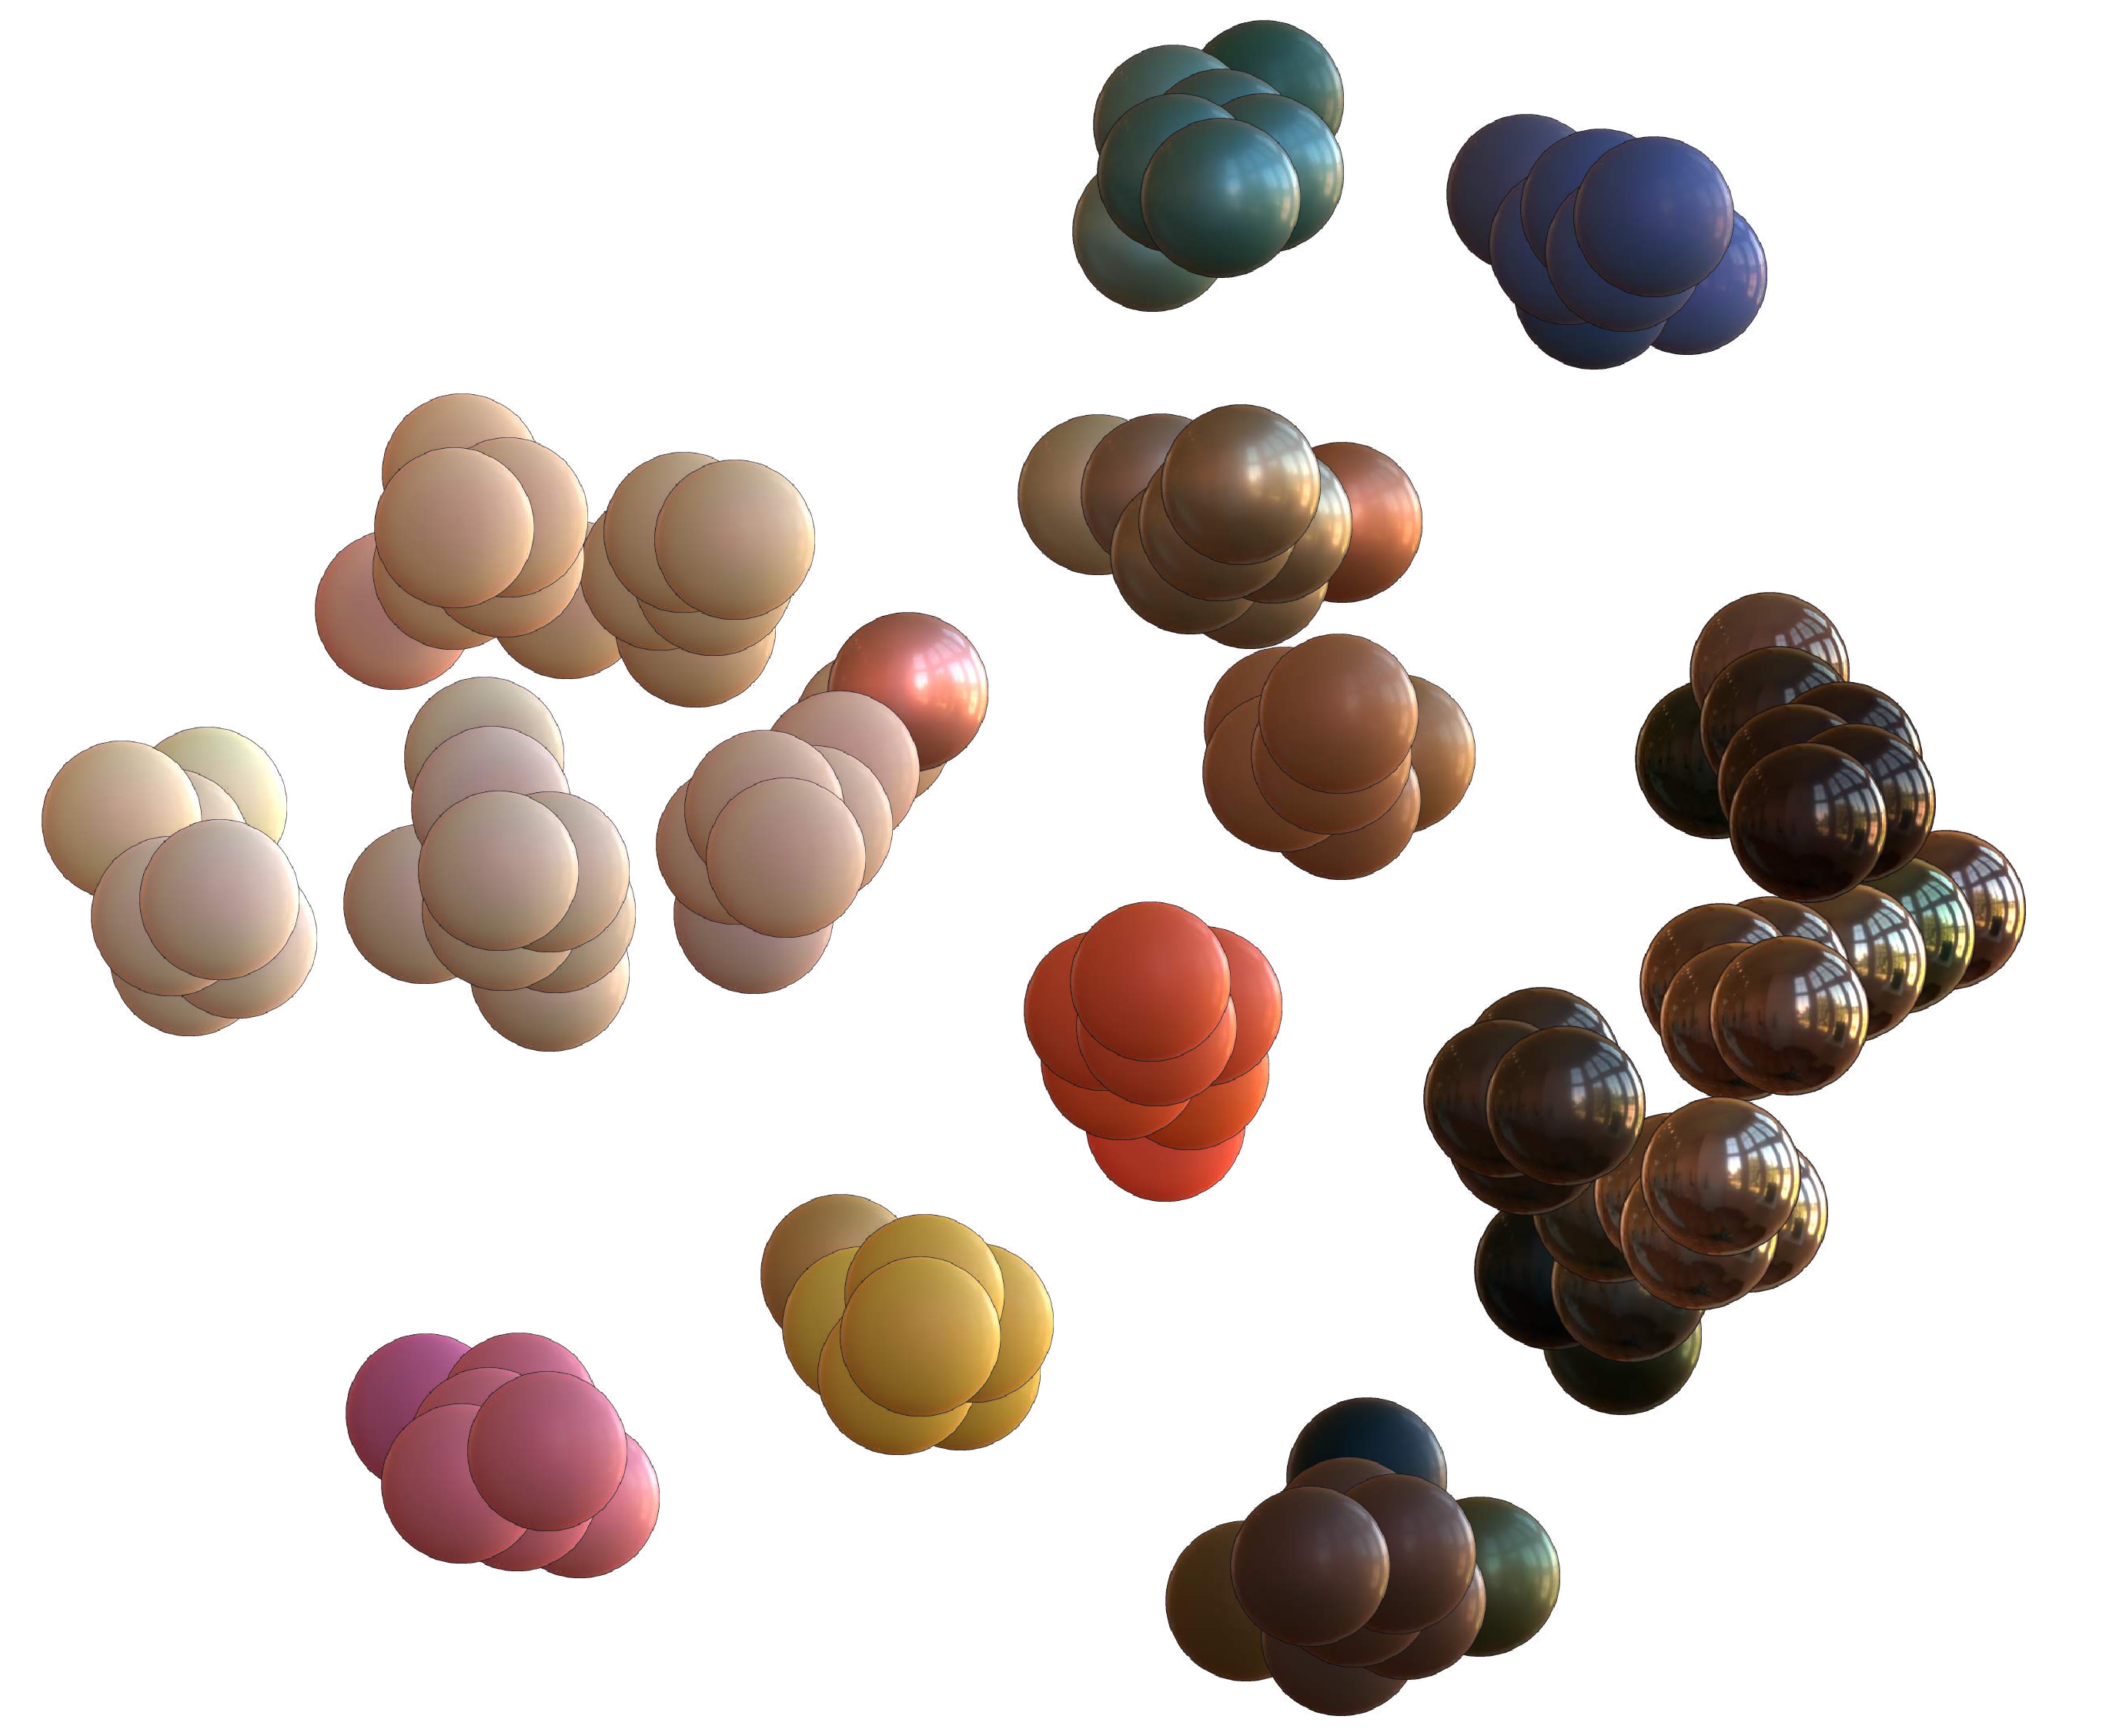
\includegraphics[width=0.8\linewidth]{Chapters/hyperbrdf-figs/tsne6_2_den1-cropped-compressed.pdf}
   \caption{t-SNE clustering of the test embeddings with different sample sizes, including $N=8, 40, 160, 4\,000, 40\,000, 640\,000$.}

   \label{fig:tsne-vis-imputation}
\end{figure}


\subsubsection{Qualitative comparison}\label{sec:qual_comp}
\begin{figure*}[t]
  \centering
%\adjustbox{trim={0.\width} {.\height} {0.89\width} {.\height},clip}%
  %{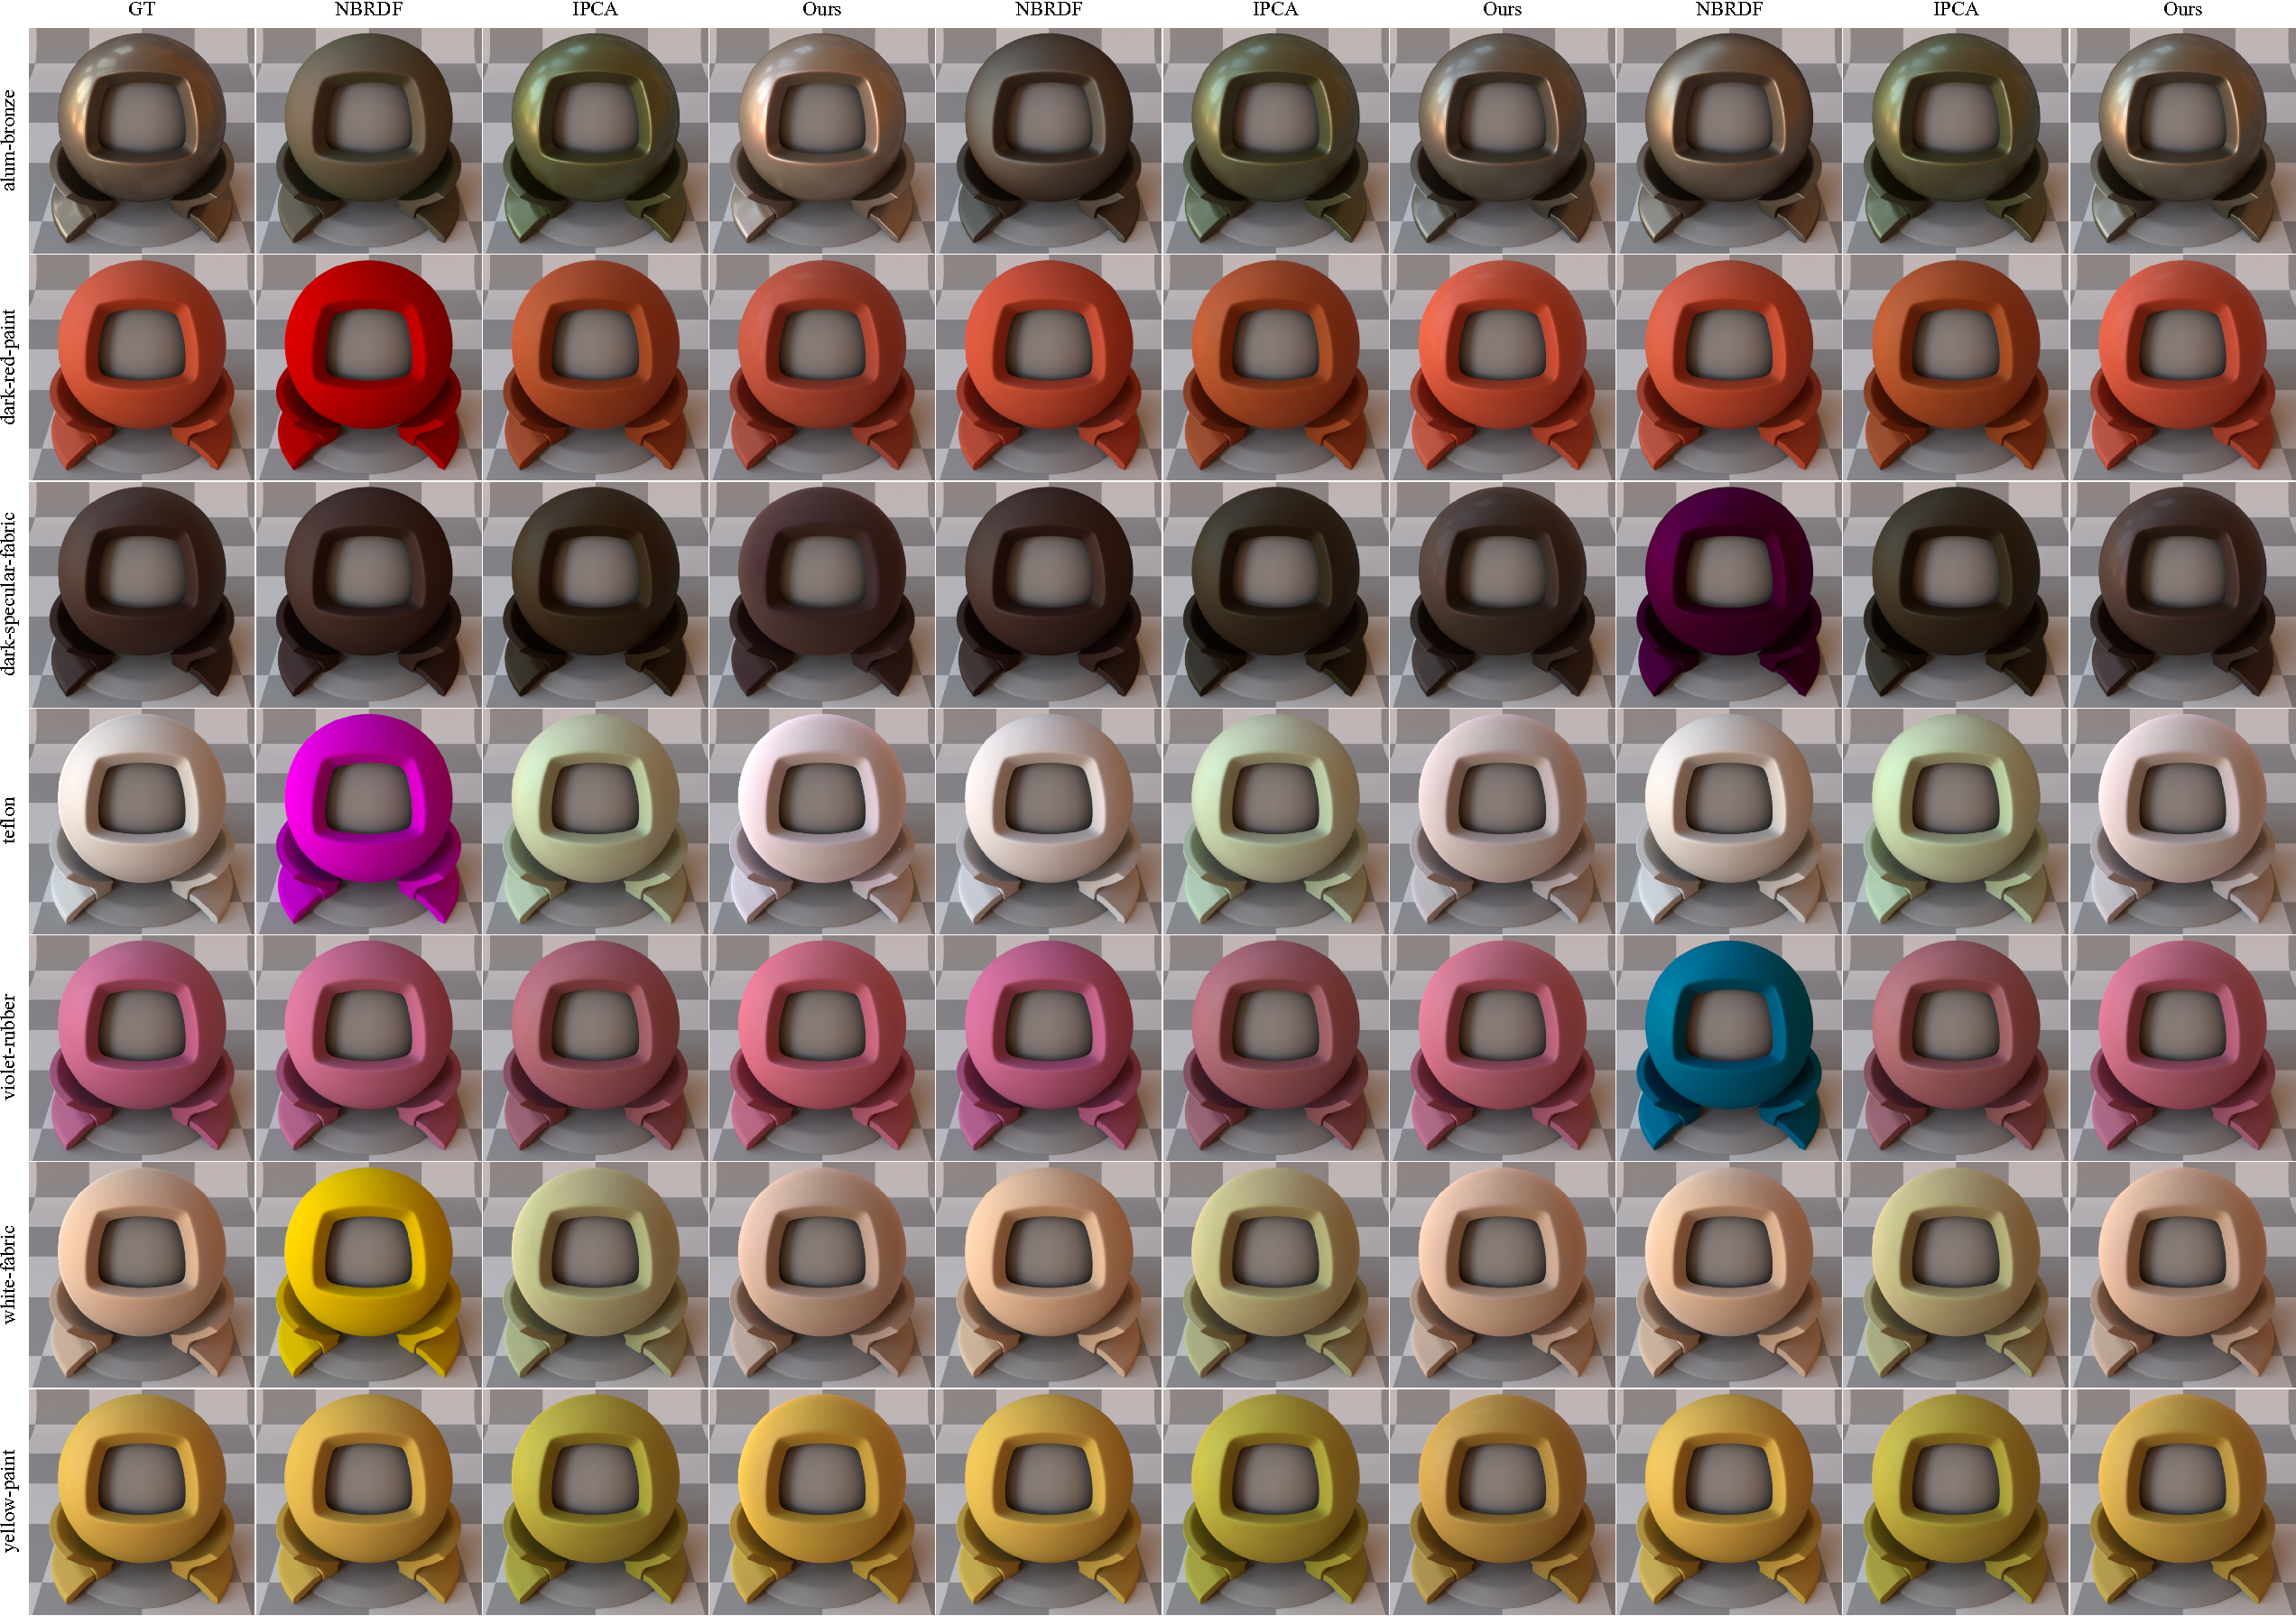
\includegraphics[width=0.9\linewidth]{Chapters/hyperbrdf-figs/imp_comp_upt_3vals.pdf}}
%\adjustbox{trim={0.113\width} {.\height} {0.596\width} {.\height},clip}%
  %{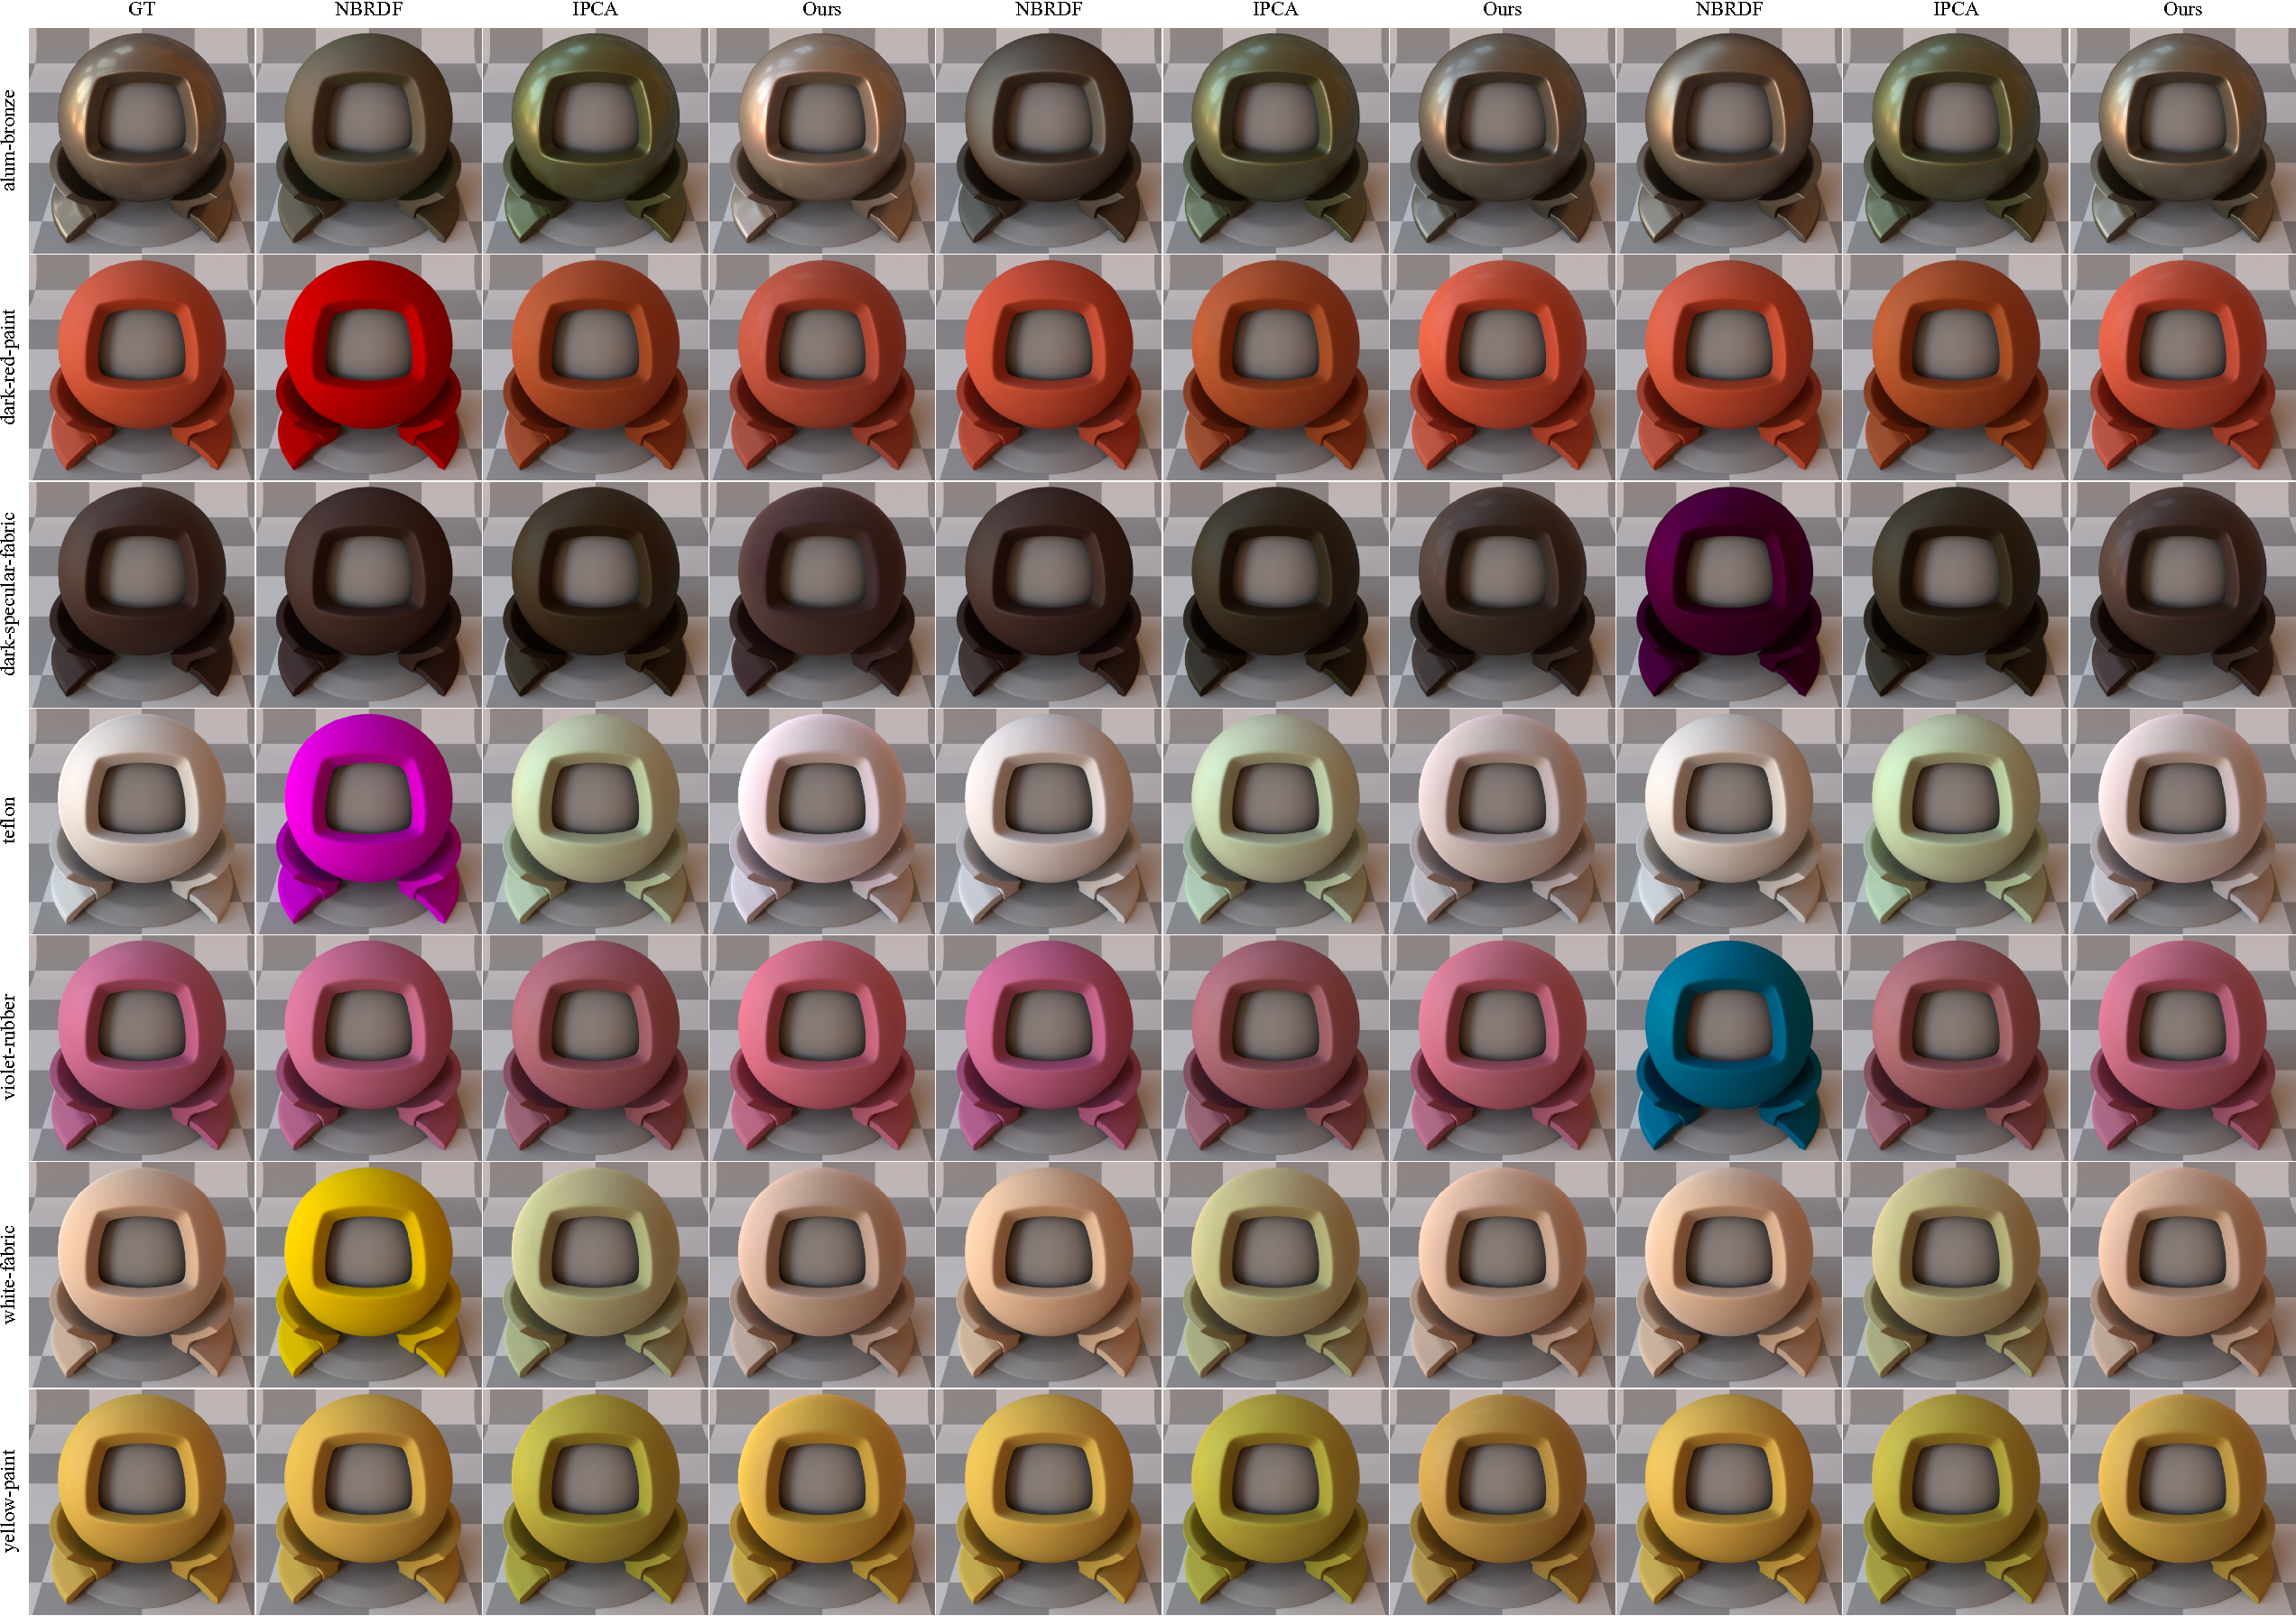
\includegraphics[width=0.9\linewidth]{Chapters/hyperbrdf-figs/imp_comp_upt_3vals.pdf}}
%\adjustbox{trim={0.41\width} {.\height} {0.298\width} {.\height},clip}%
  %{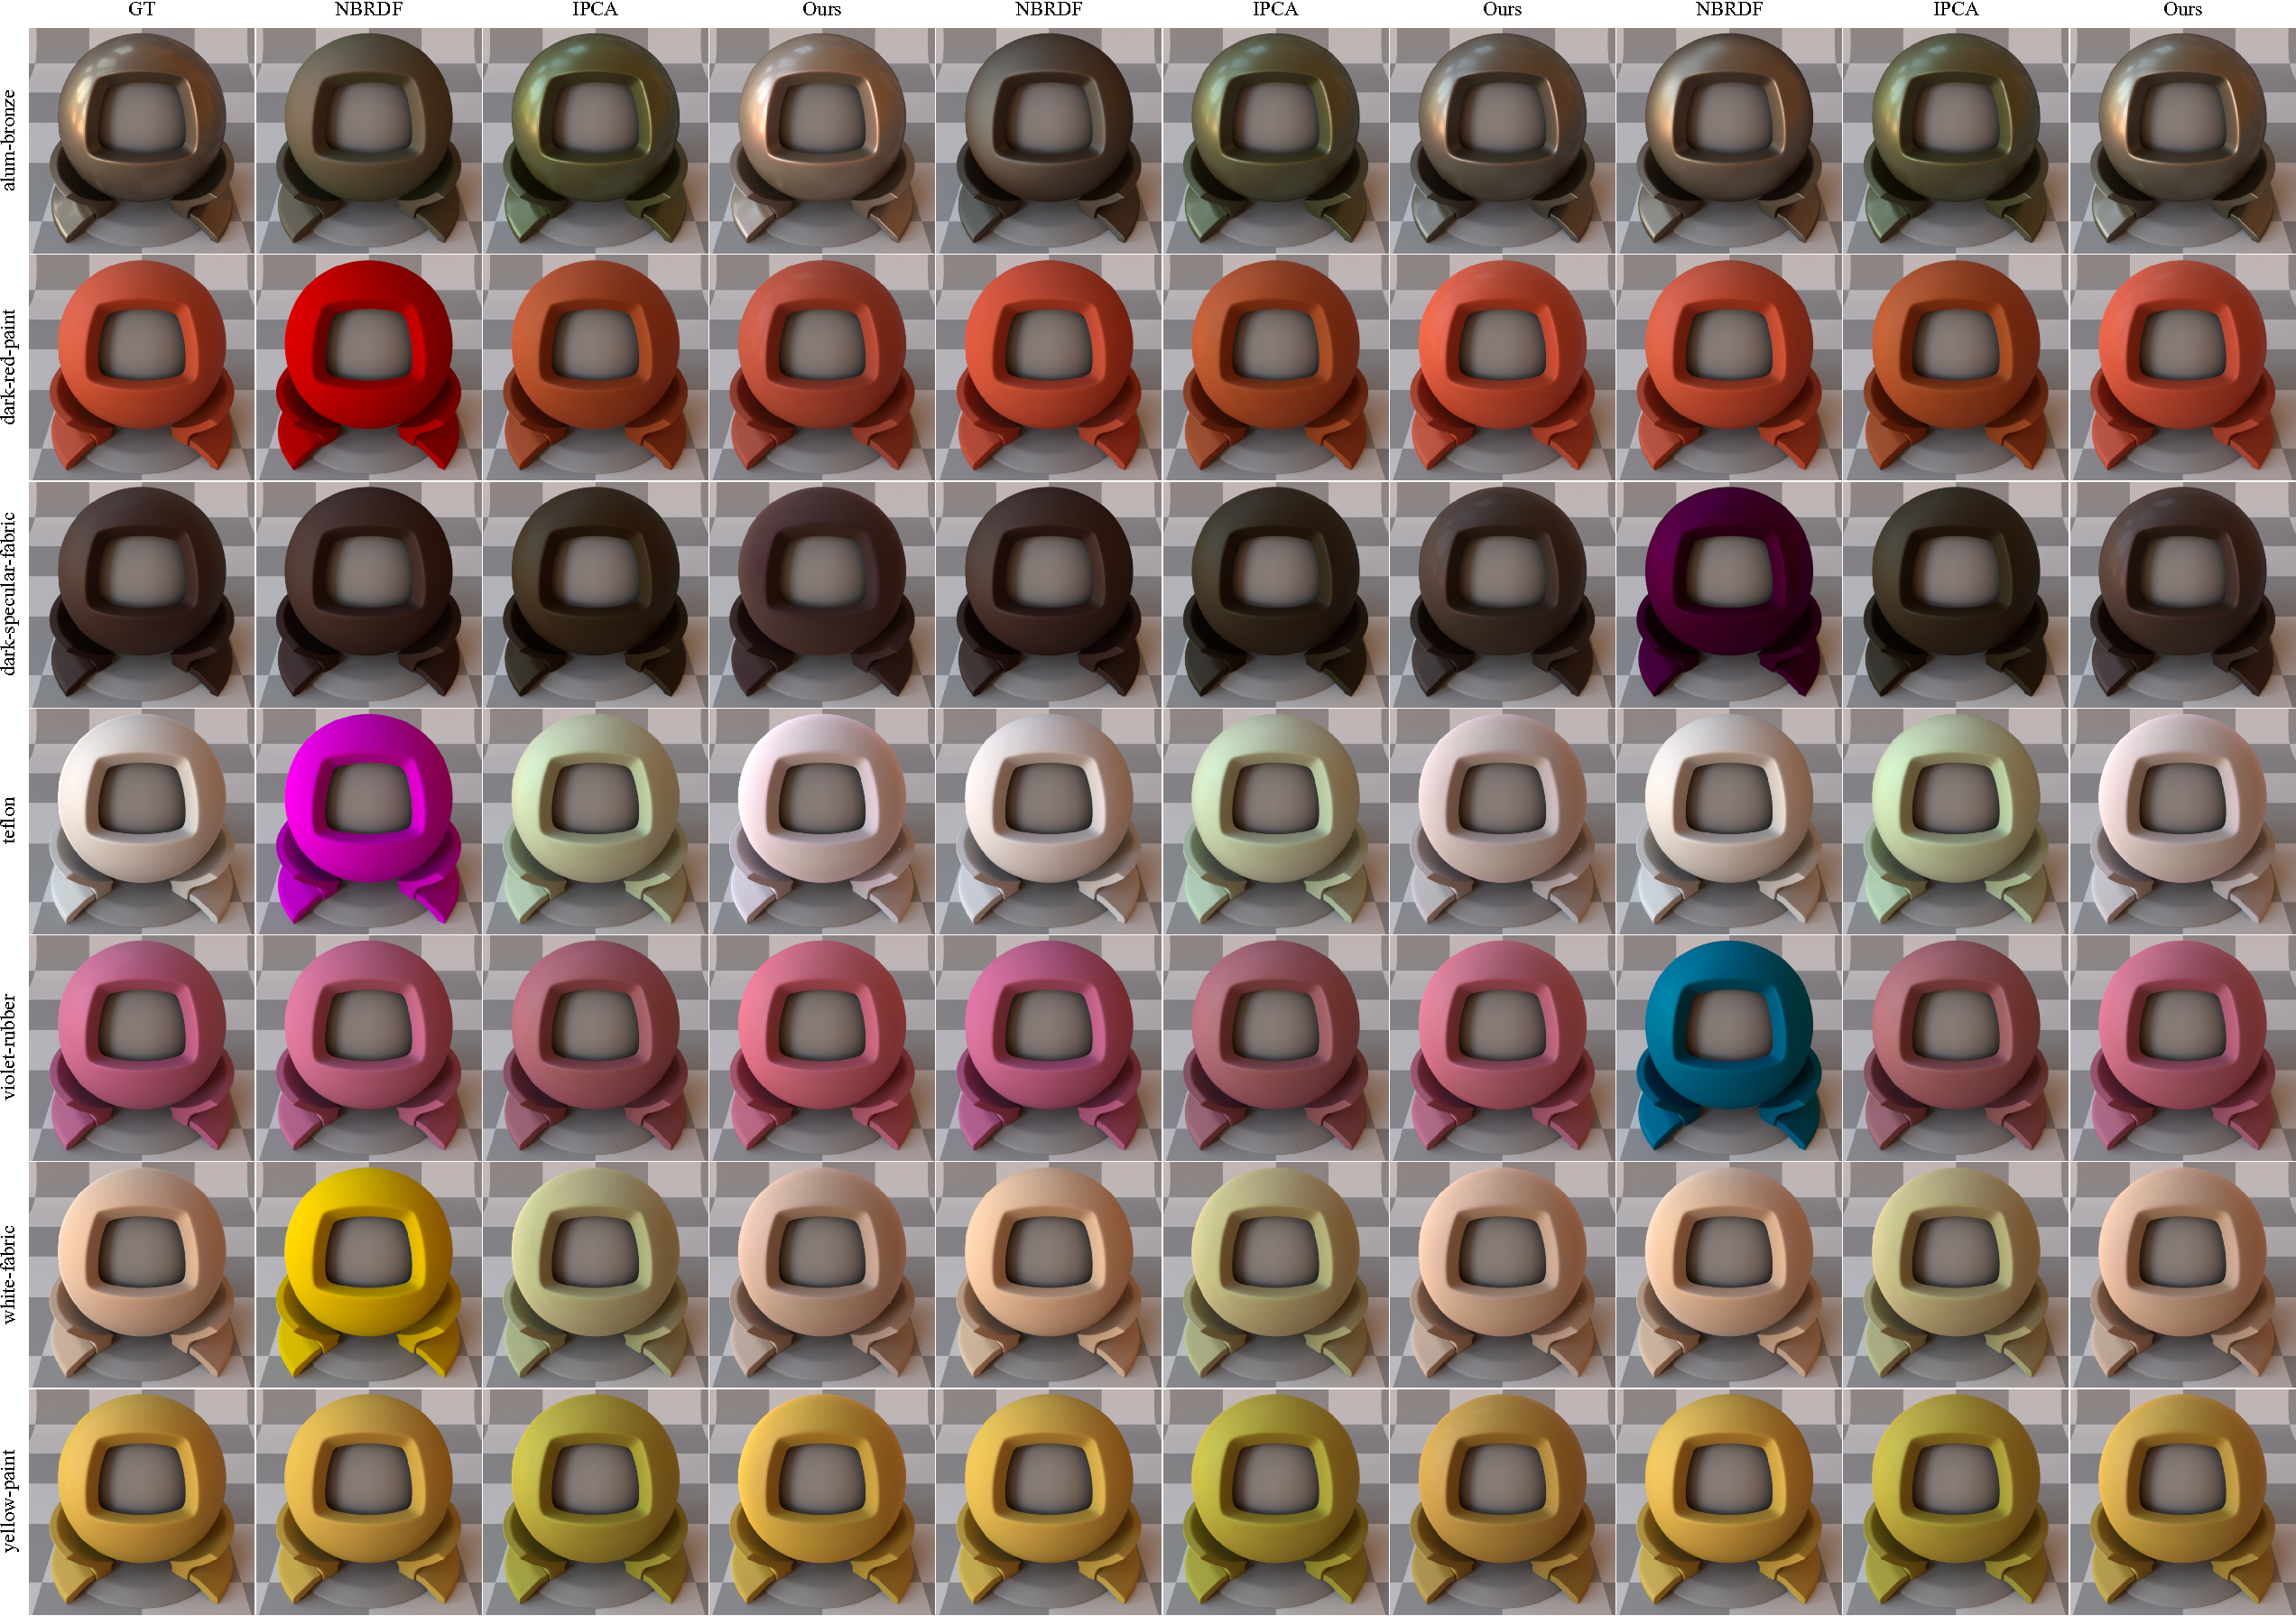
\includegraphics[width=0.9\linewidth]{Chapters/hyperbrdf-figs/imp_comp_upt_3vals.pdf}}
%\adjustbox{trim={0.707\width} {.\height} {0.\width} {.\height},clip}%
 % {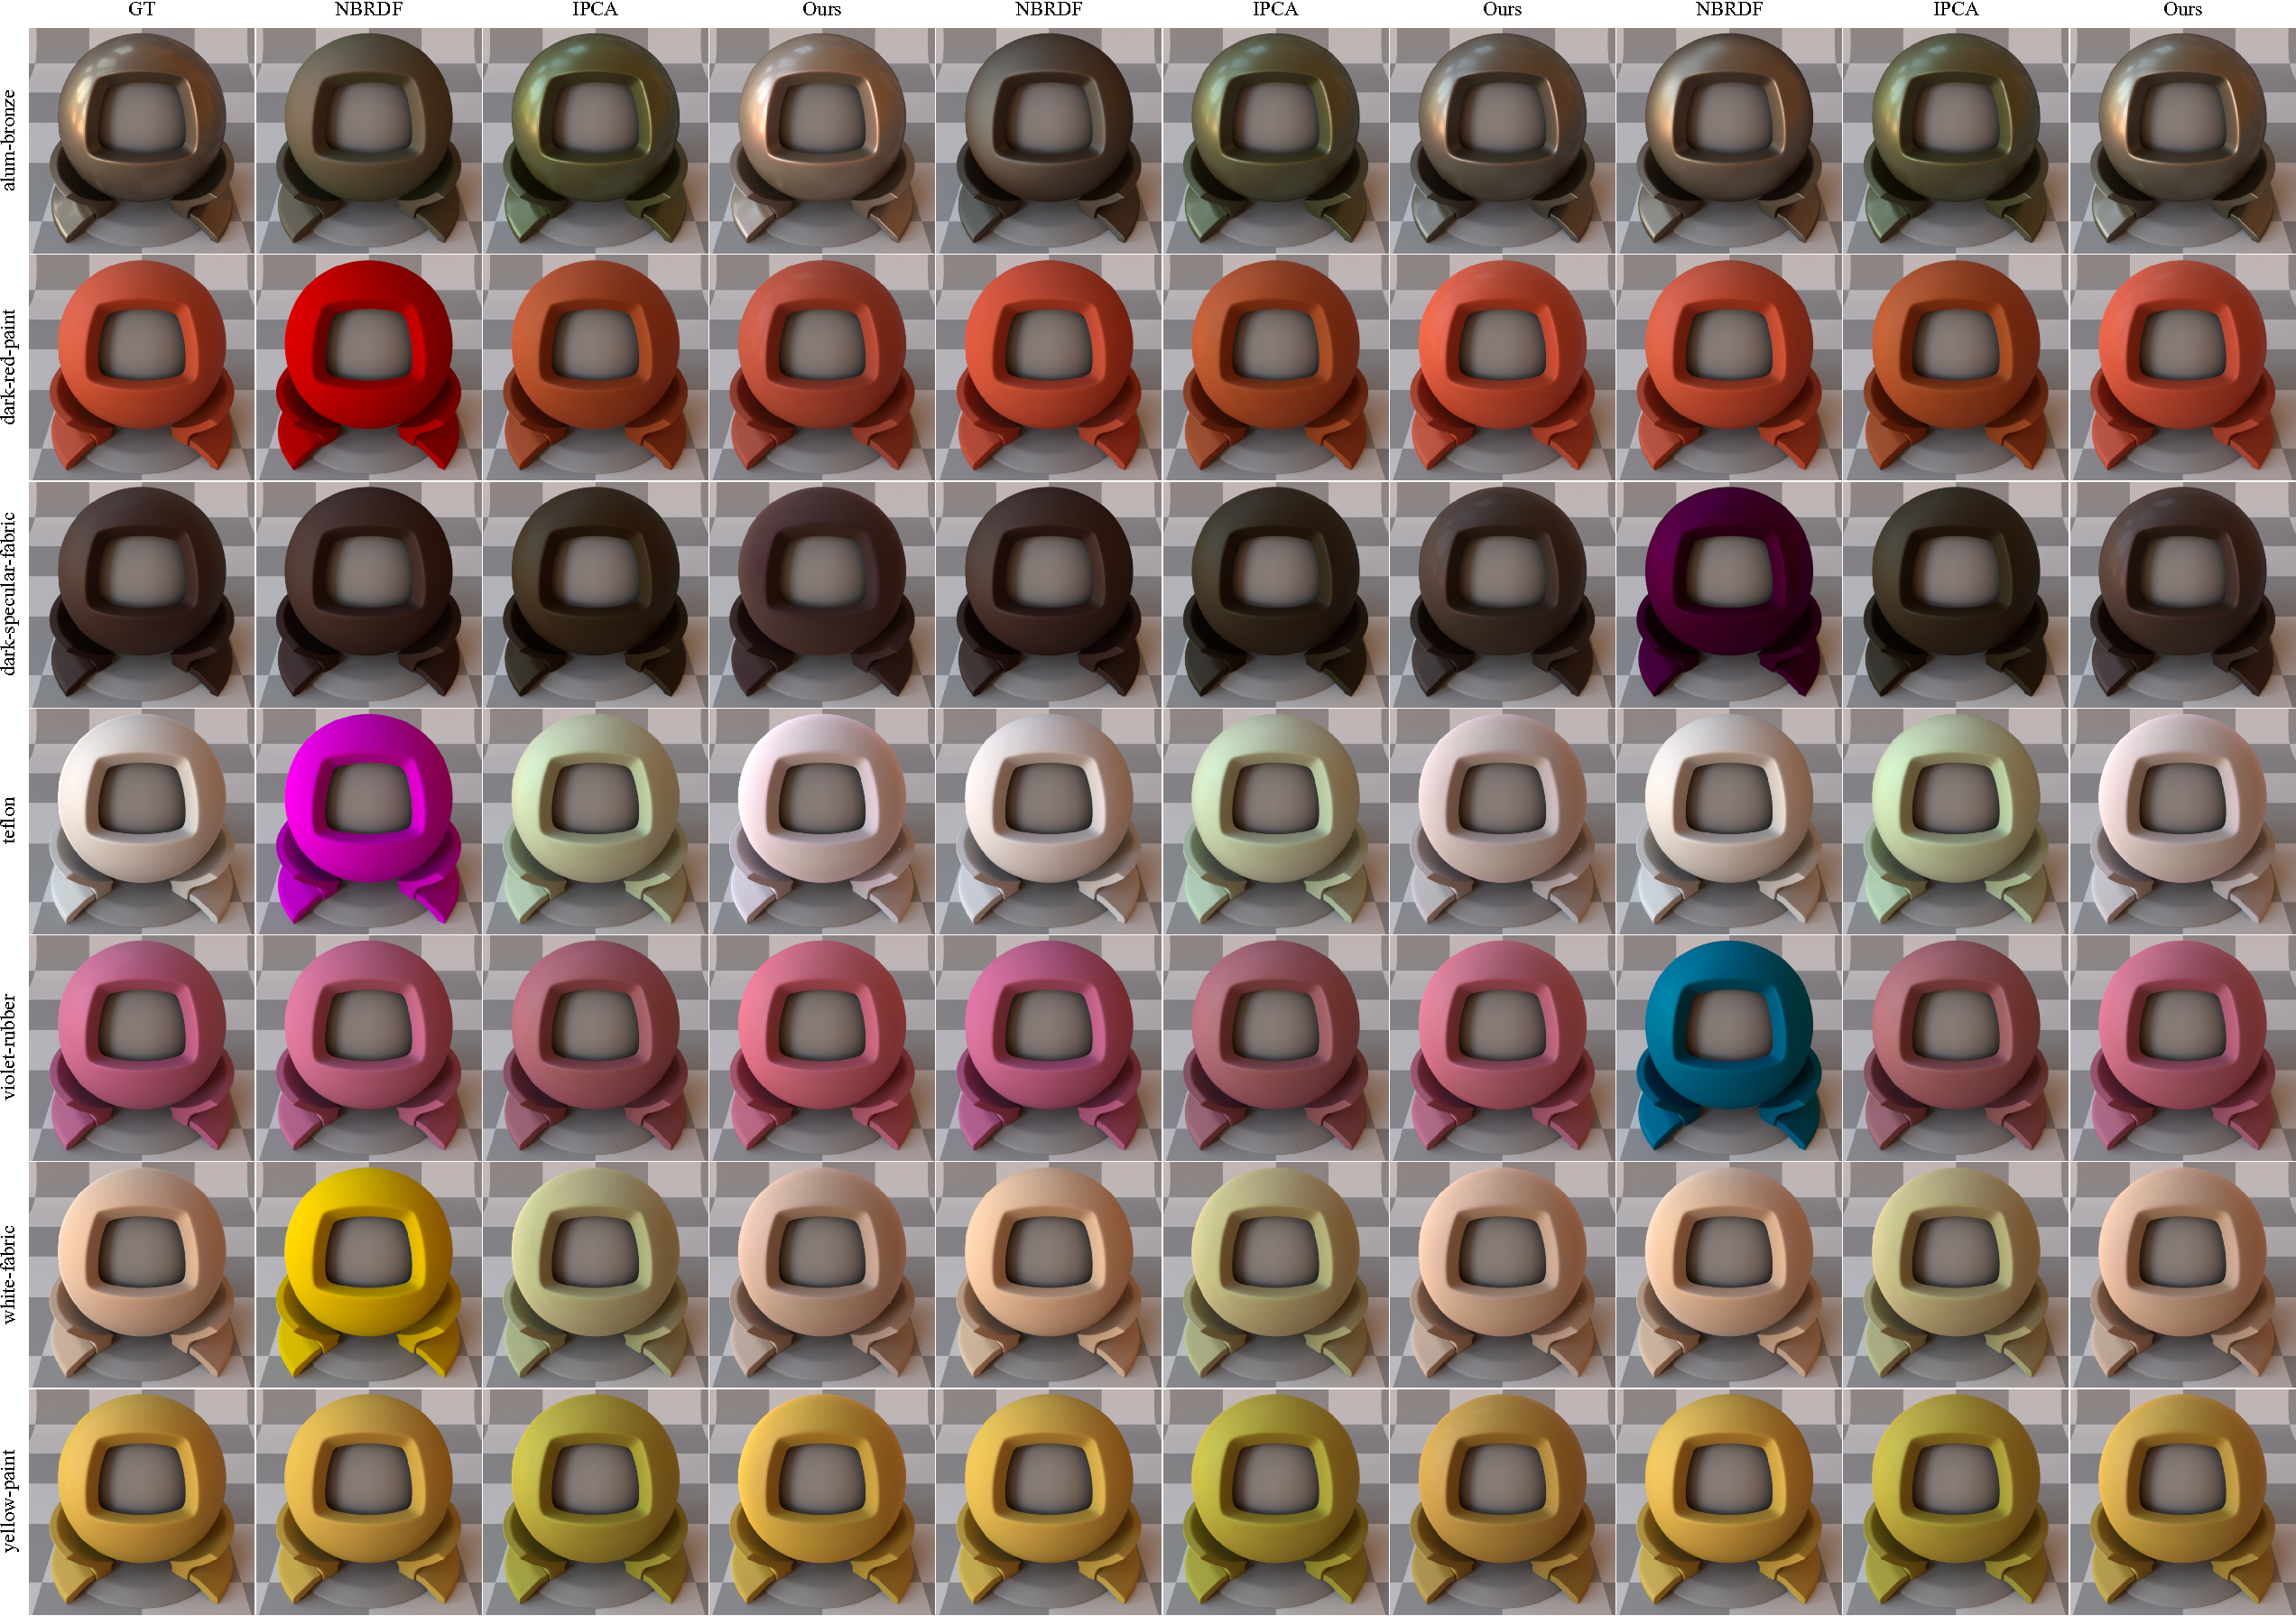
\includegraphics[width=0.9\linewidth]{Chapters/hyperbrdf-figs/imp_comp_upt_3vals.pdf}}

%\adjustbox{trim={0.\width} {.\height} {0.89\width} {.06\height},clip}%
  %{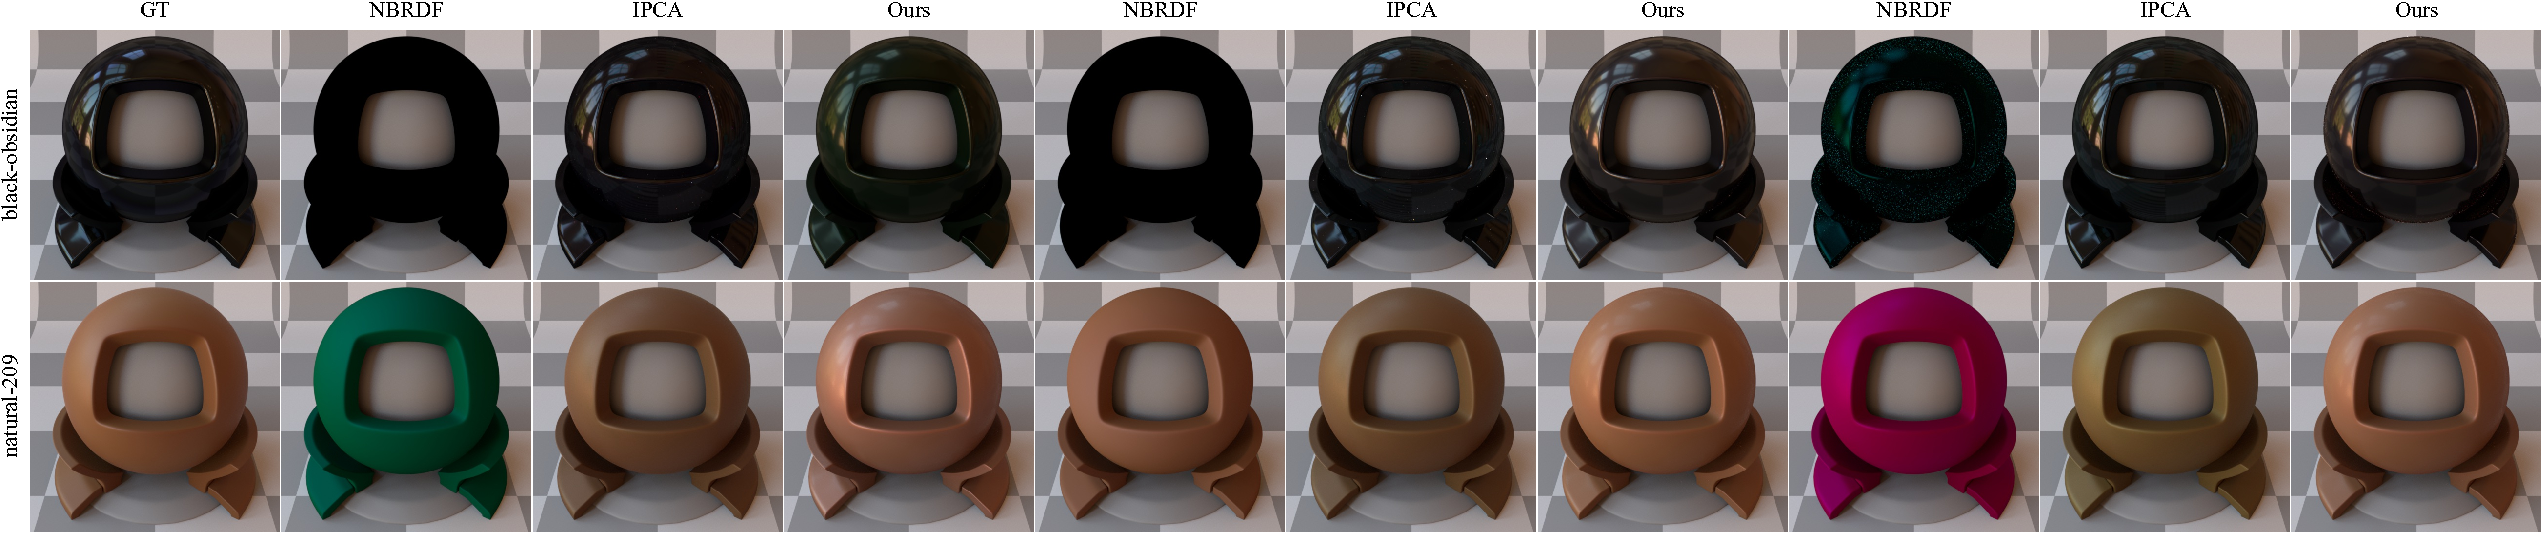
\includegraphics[width=0.9\linewidth]{Chapters/hyperbrdf-figs/imp_comp_upt_3vals_bad.pdf}}
%\adjustbox{trim={0.113\width} {.\height} {0.596\width} {.06\height},clip}%
  %{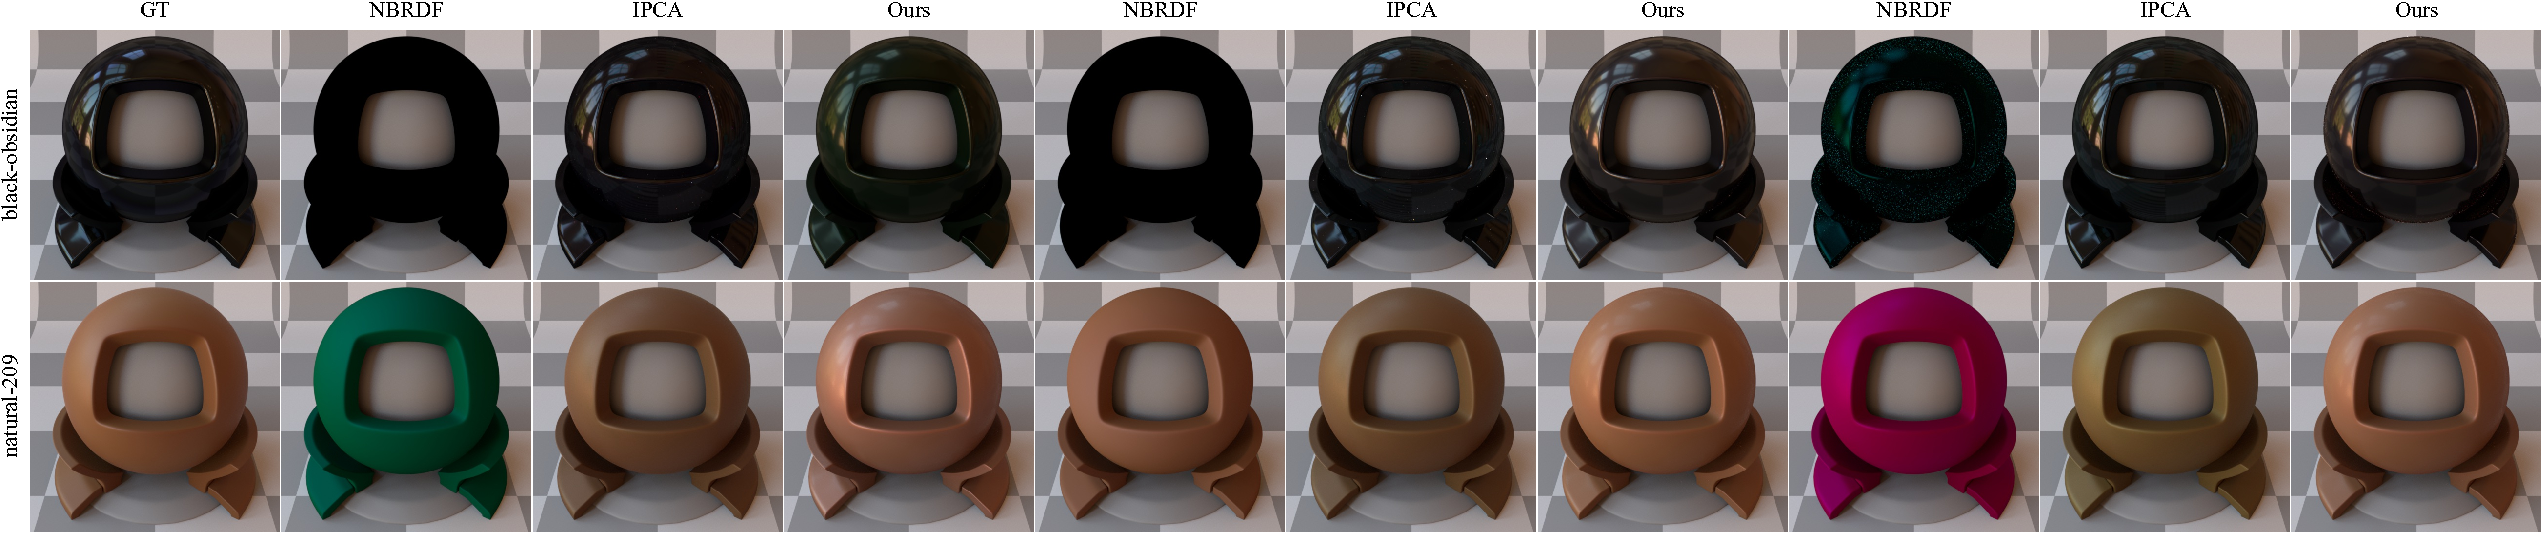
\includegraphics[width=0.9\linewidth]{Chapters/hyperbrdf-figs/imp_comp_upt_3vals_bad.pdf}}
%\adjustbox{trim={0.41\width} {.\height} {0.298\width} {.06\height},clip}%
  %{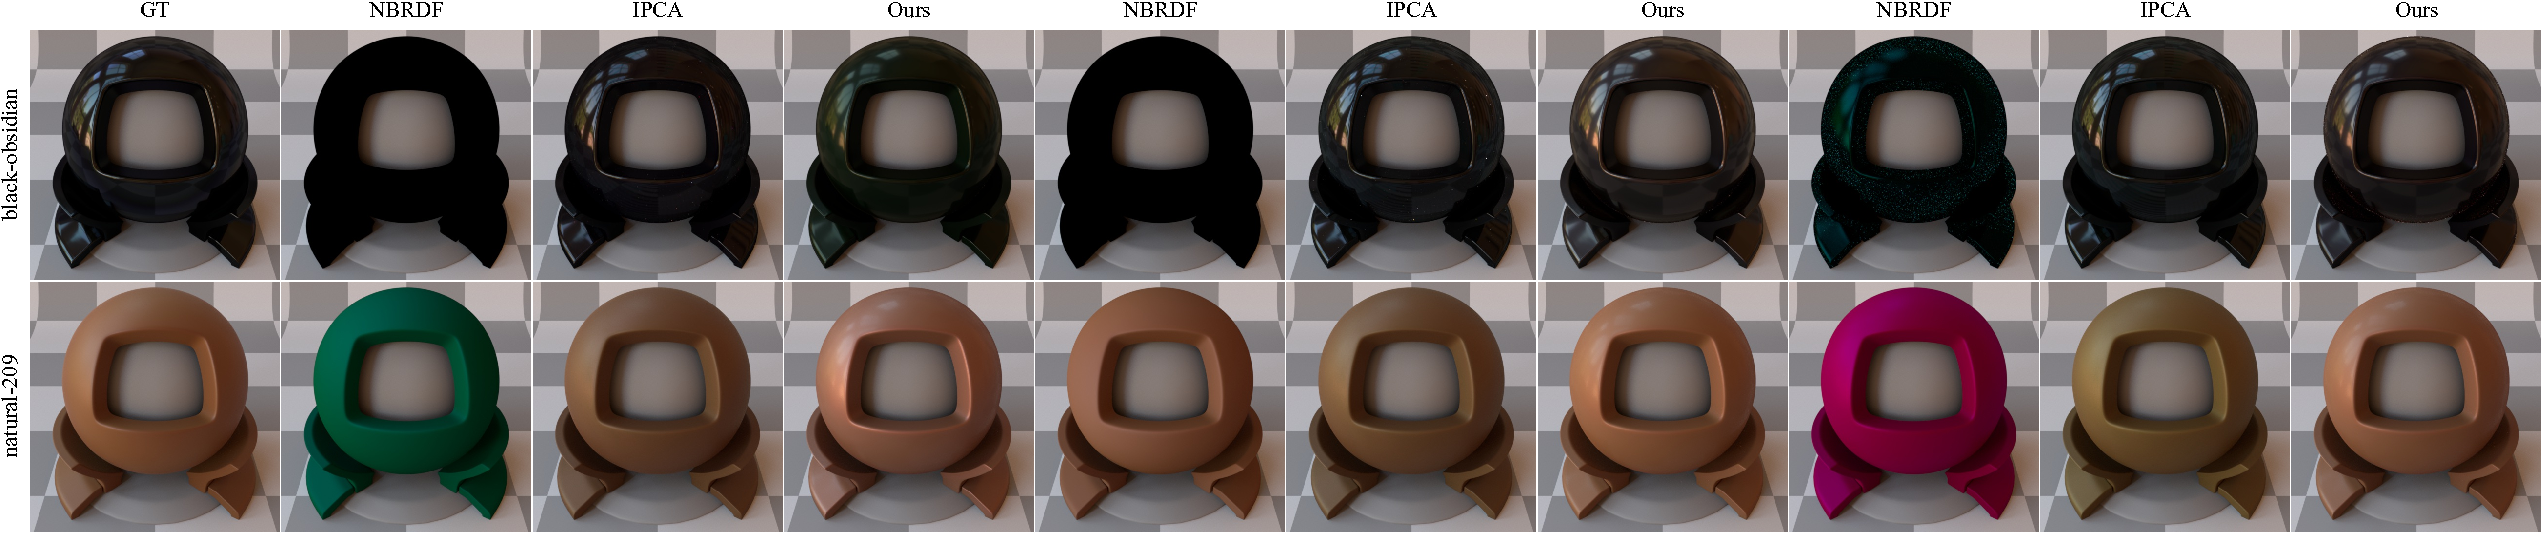
\includegraphics[width=0.9\linewidth]{Chapters/hyperbrdf-figs/imp_comp_upt_3vals_bad.pdf}}
%\adjustbox{trim={0.707\width} {.\height} {0.\width} {.06\height},clip}%
 % {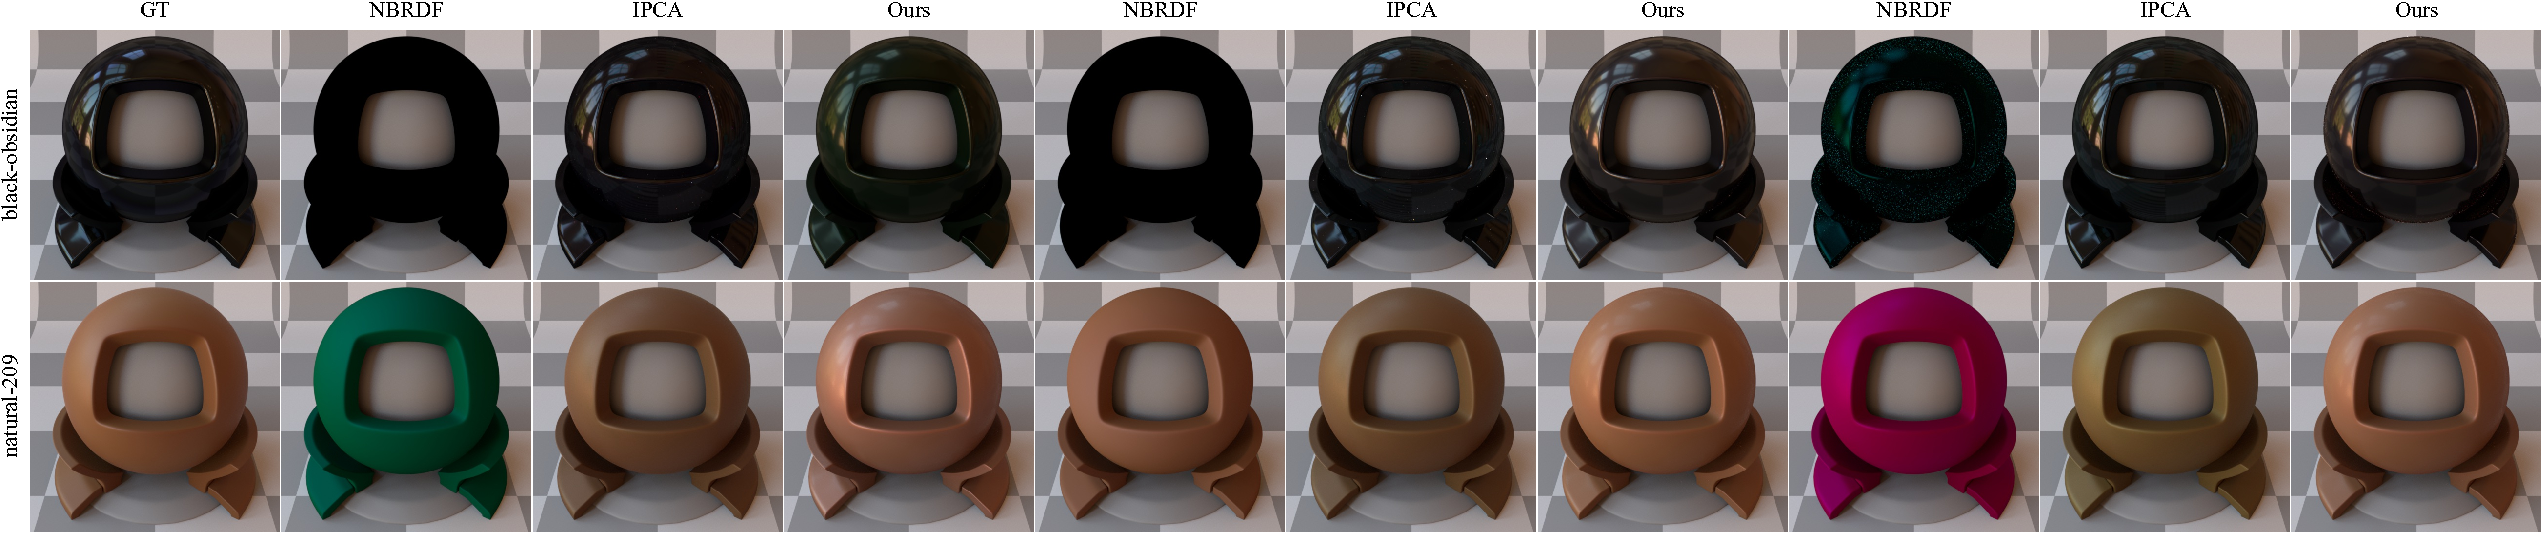
\includegraphics[width=0.9\linewidth]{Chapters/hyperbrdf-figs/imp_comp_upt_3vals_bad.pdf}}
  
  \adjustbox{trim={0.07\width} {.\height} {0.816\width} {.\height},clip}%
  {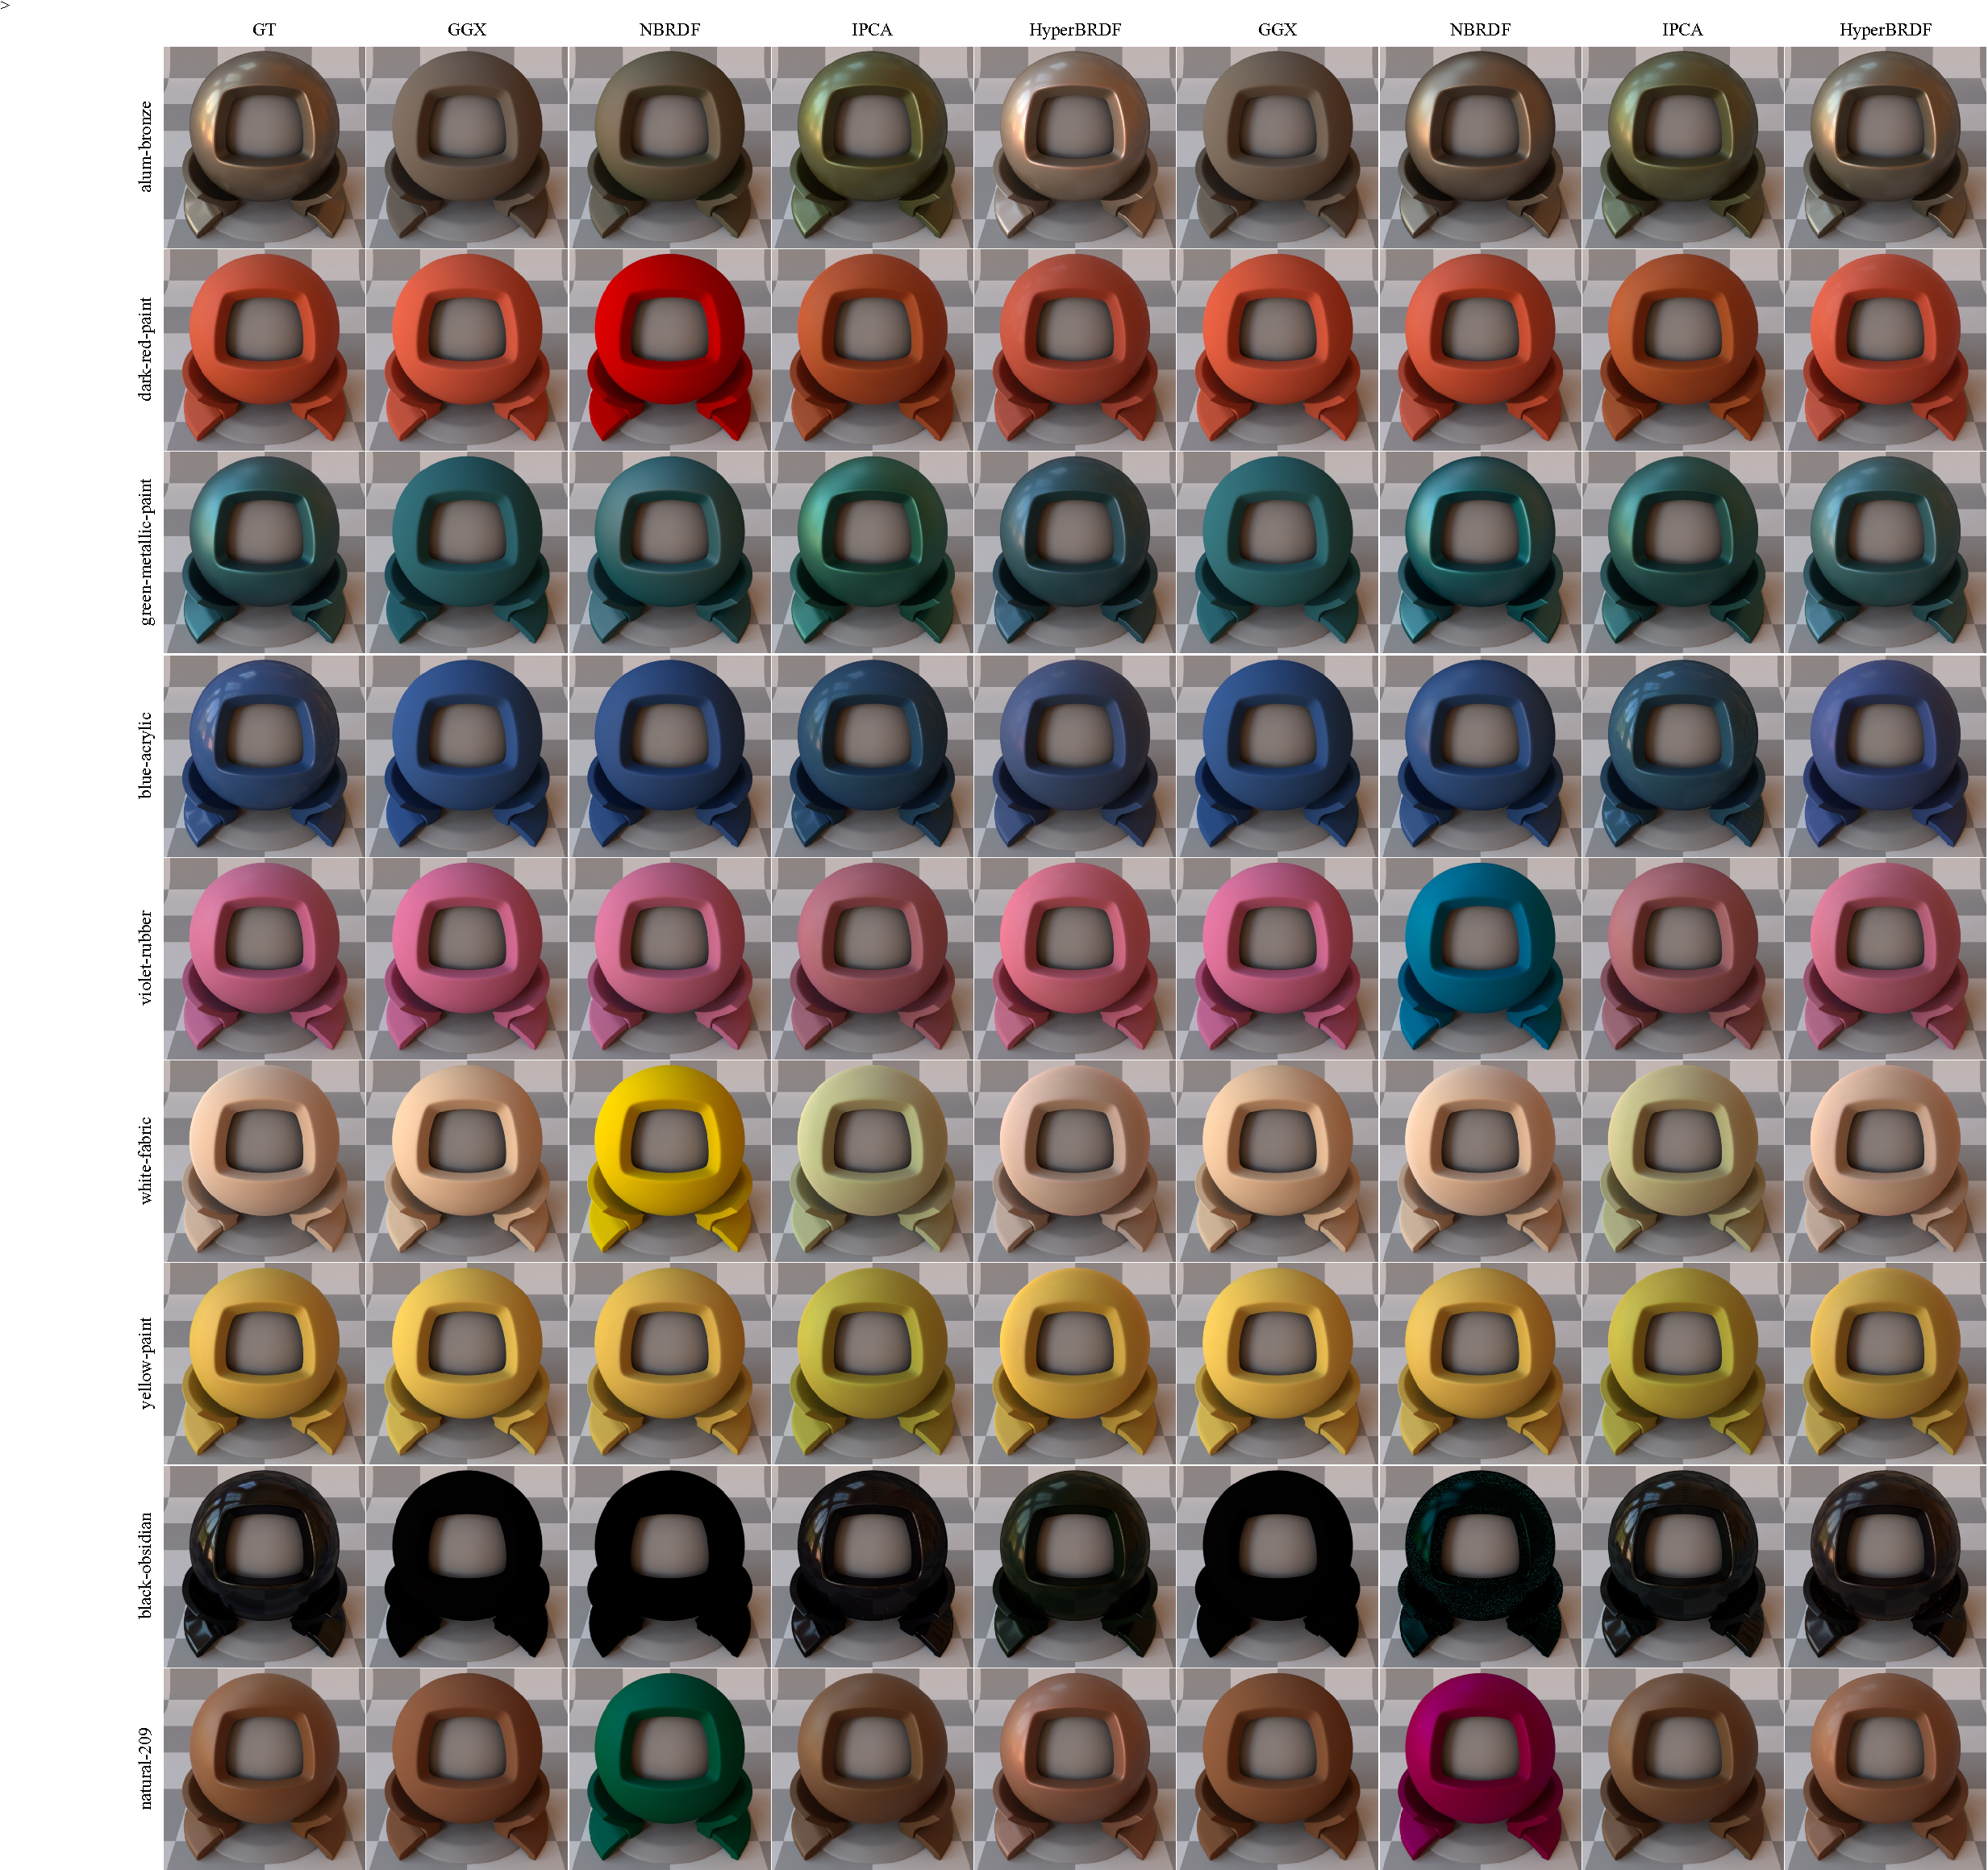
\includegraphics[width=0.9\linewidth]{Chapters/hyperbrdf-figs/qual_comp_ggx_2.pdf}}
\adjustbox{trim={0.184\width} {.\height} {0.41\width} {.\height},clip}%
{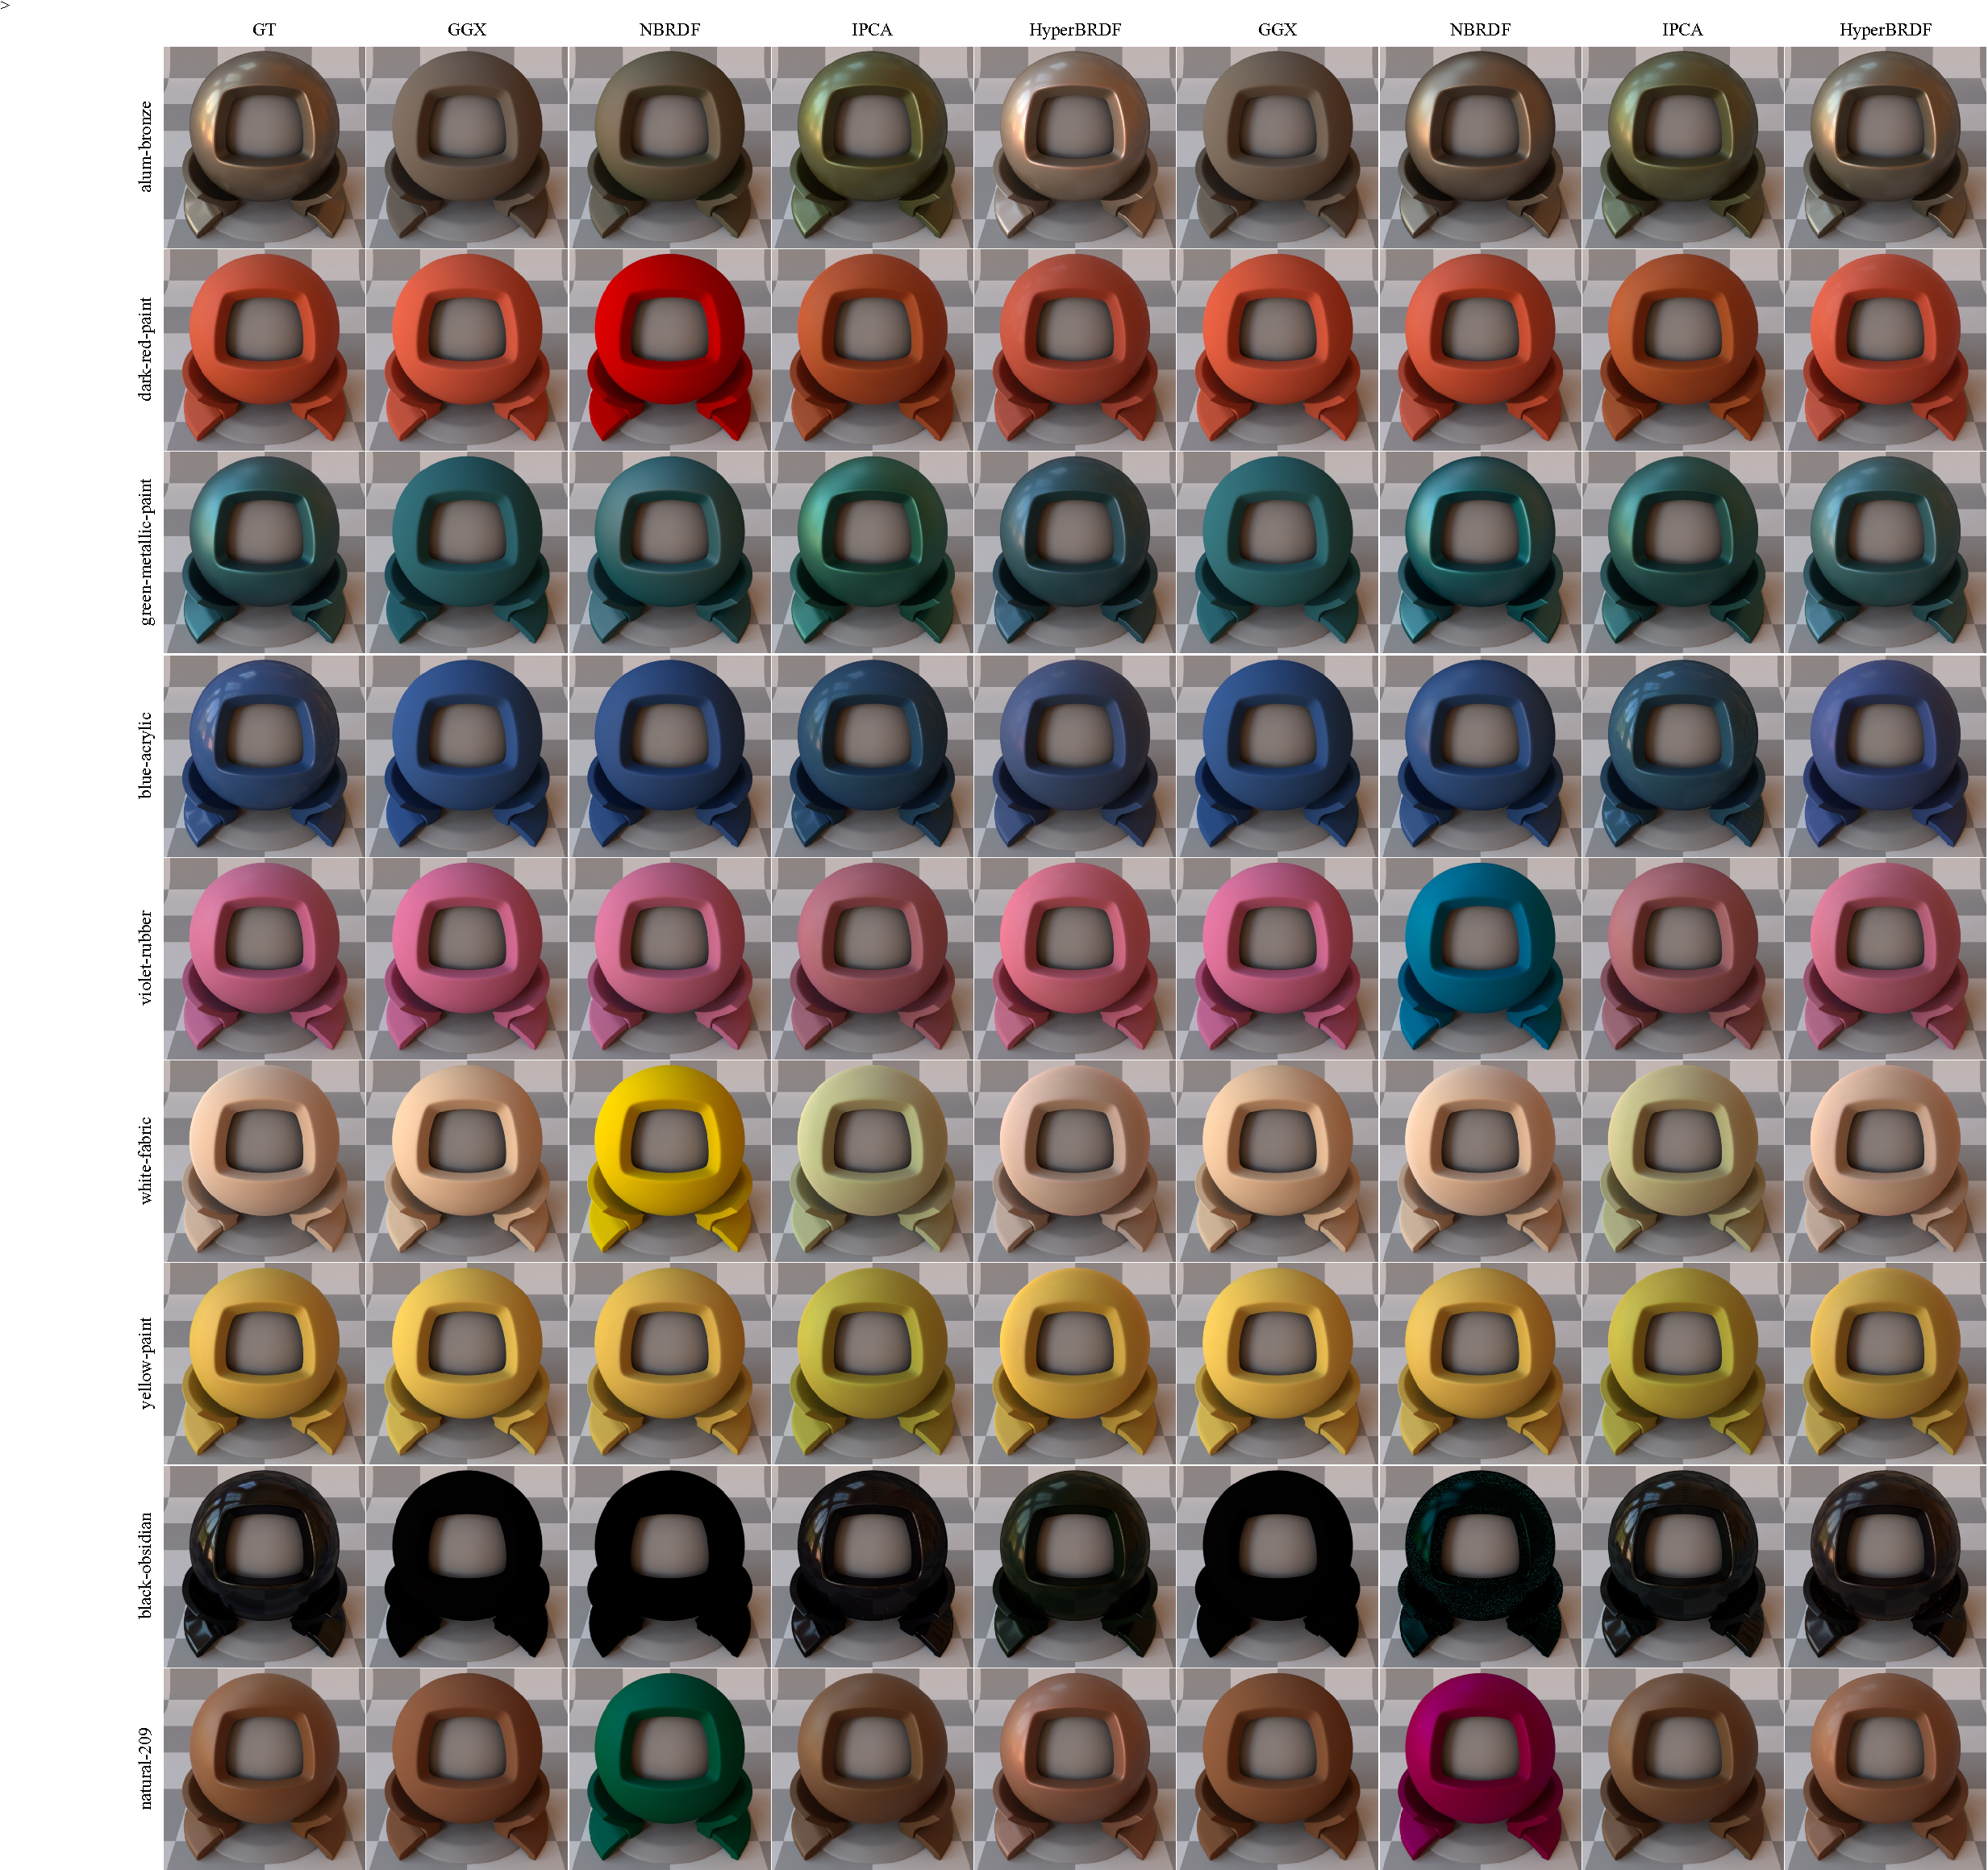
\includegraphics[width=0.9\linewidth]{Chapters/hyperbrdf-figs/qual_comp_ggx_2.pdf}}
\adjustbox{trim={0.593\width} {.\height} {0.\width} {.\height},clip}%
  {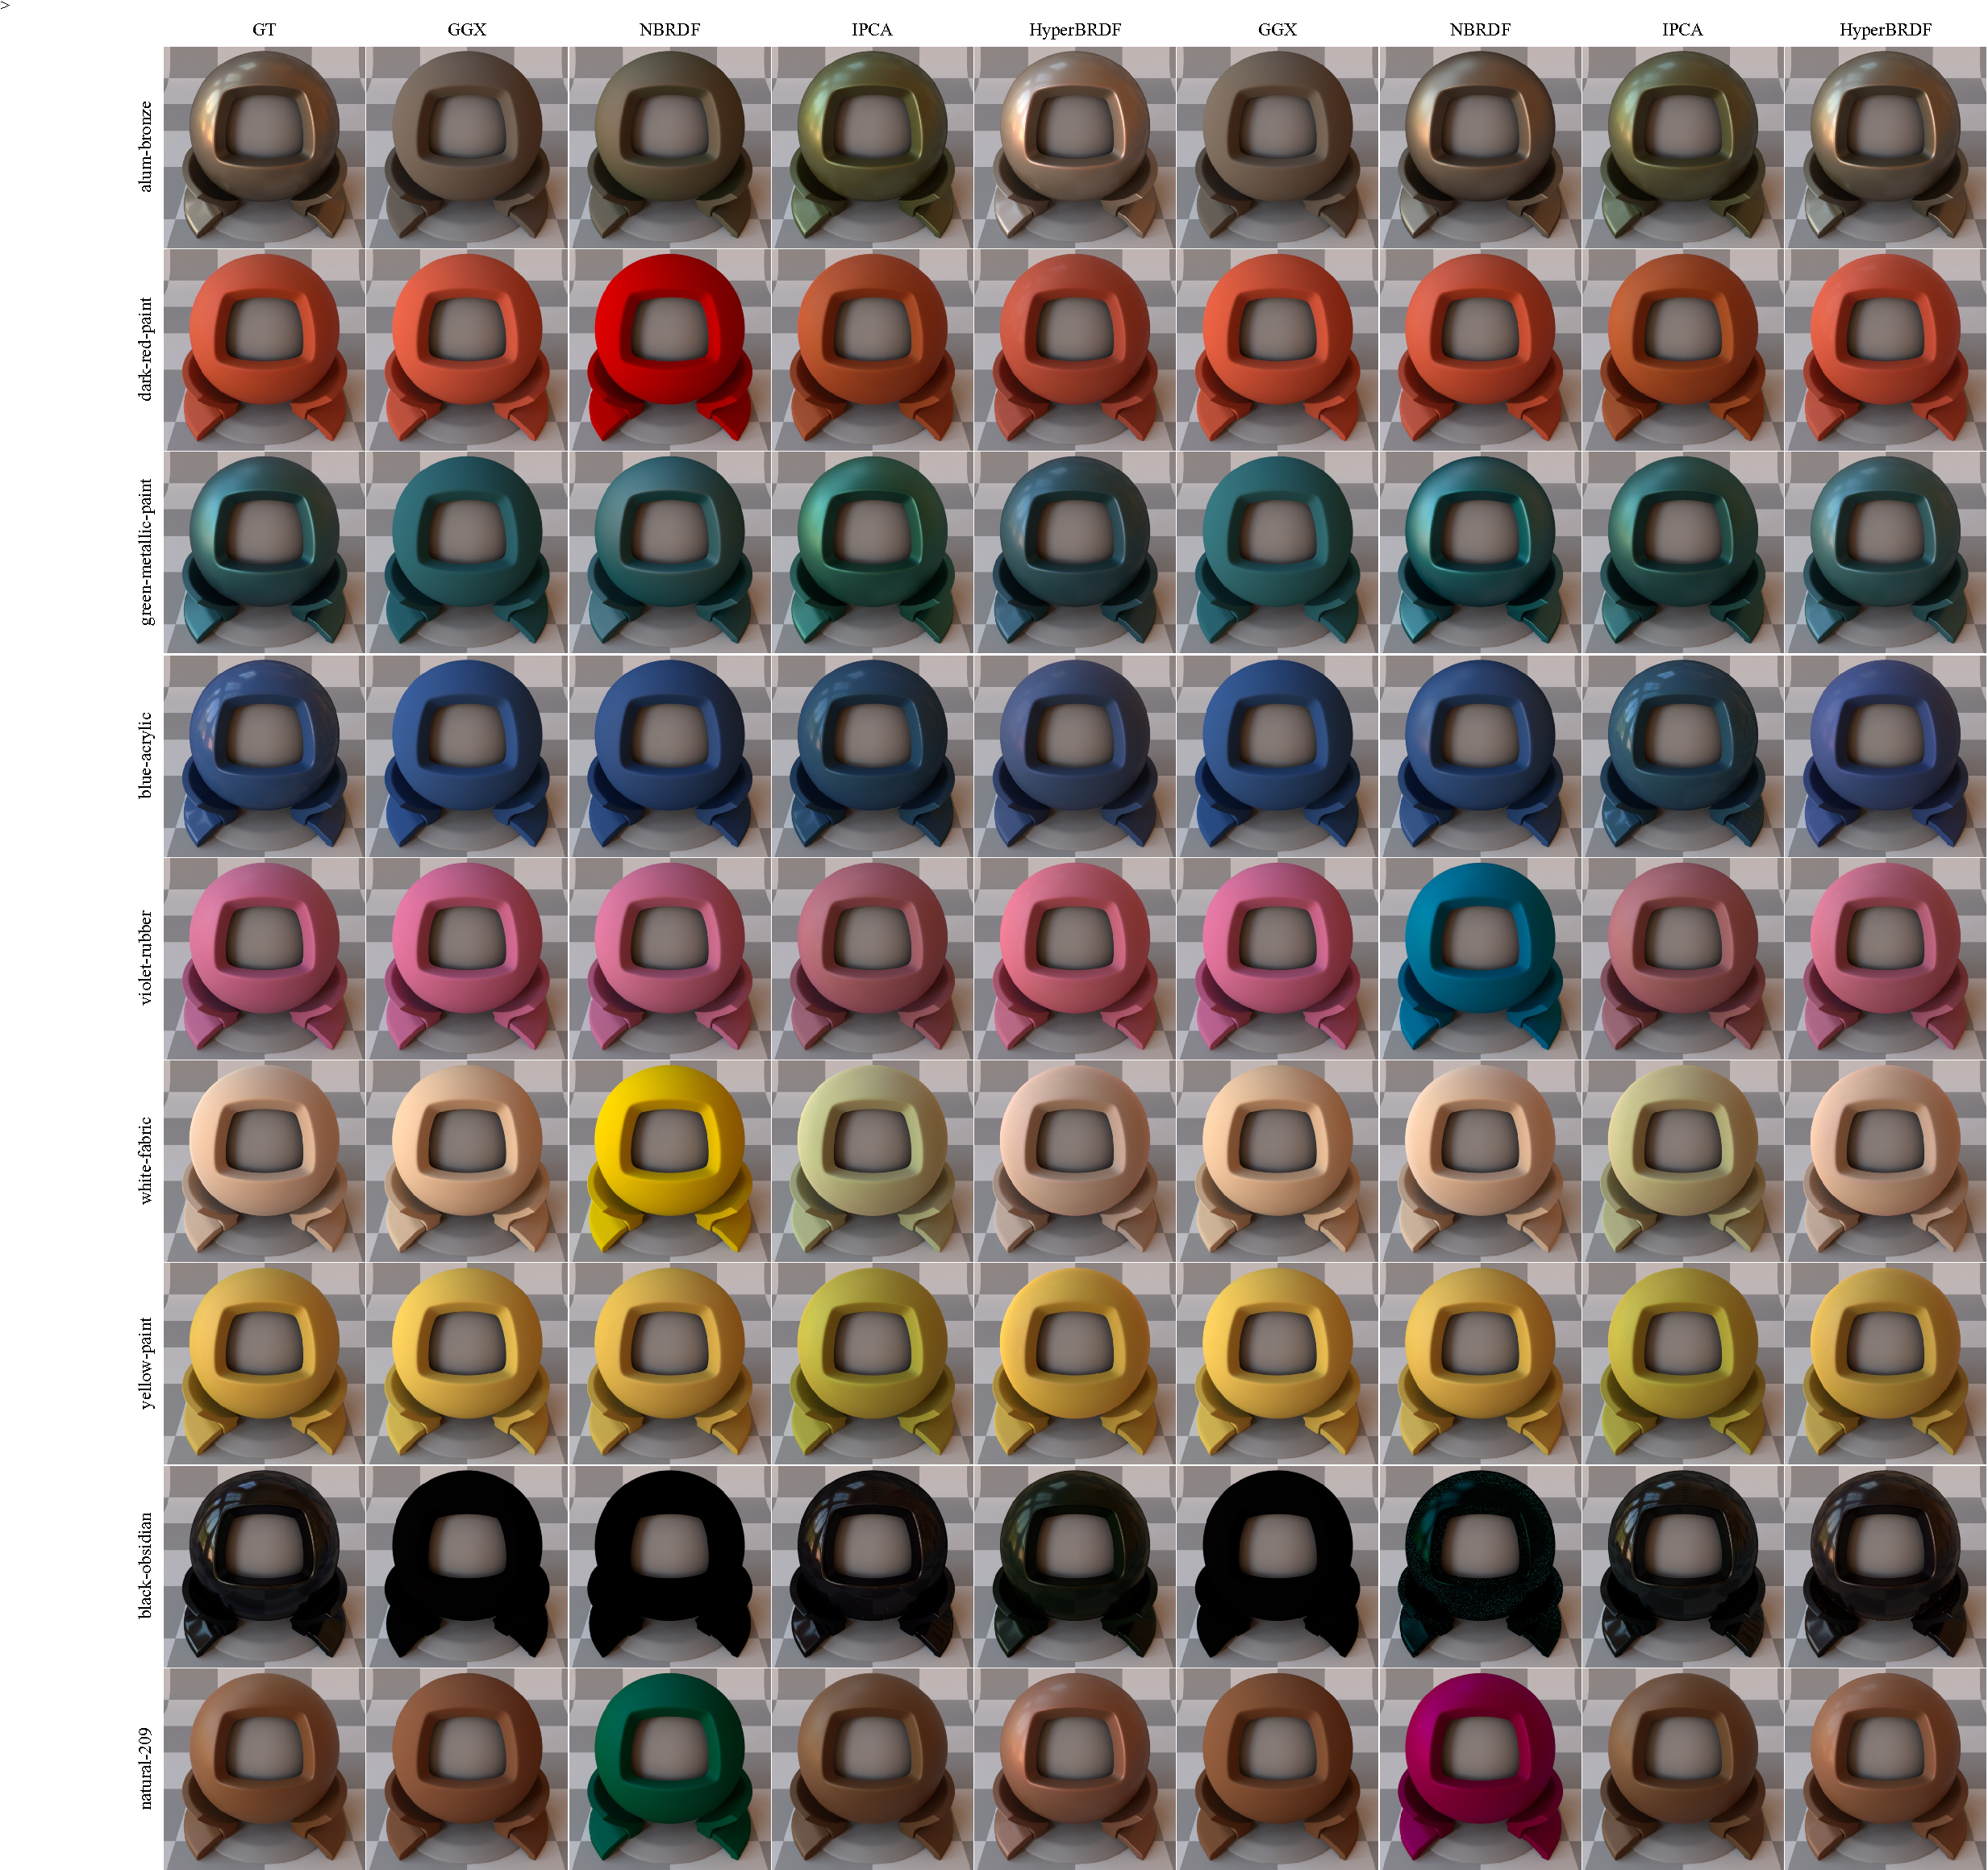
\includegraphics[width=0.9\linewidth]{Chapters/hyperbrdf-figs/qual_comp_ggx_2.pdf}}
 %{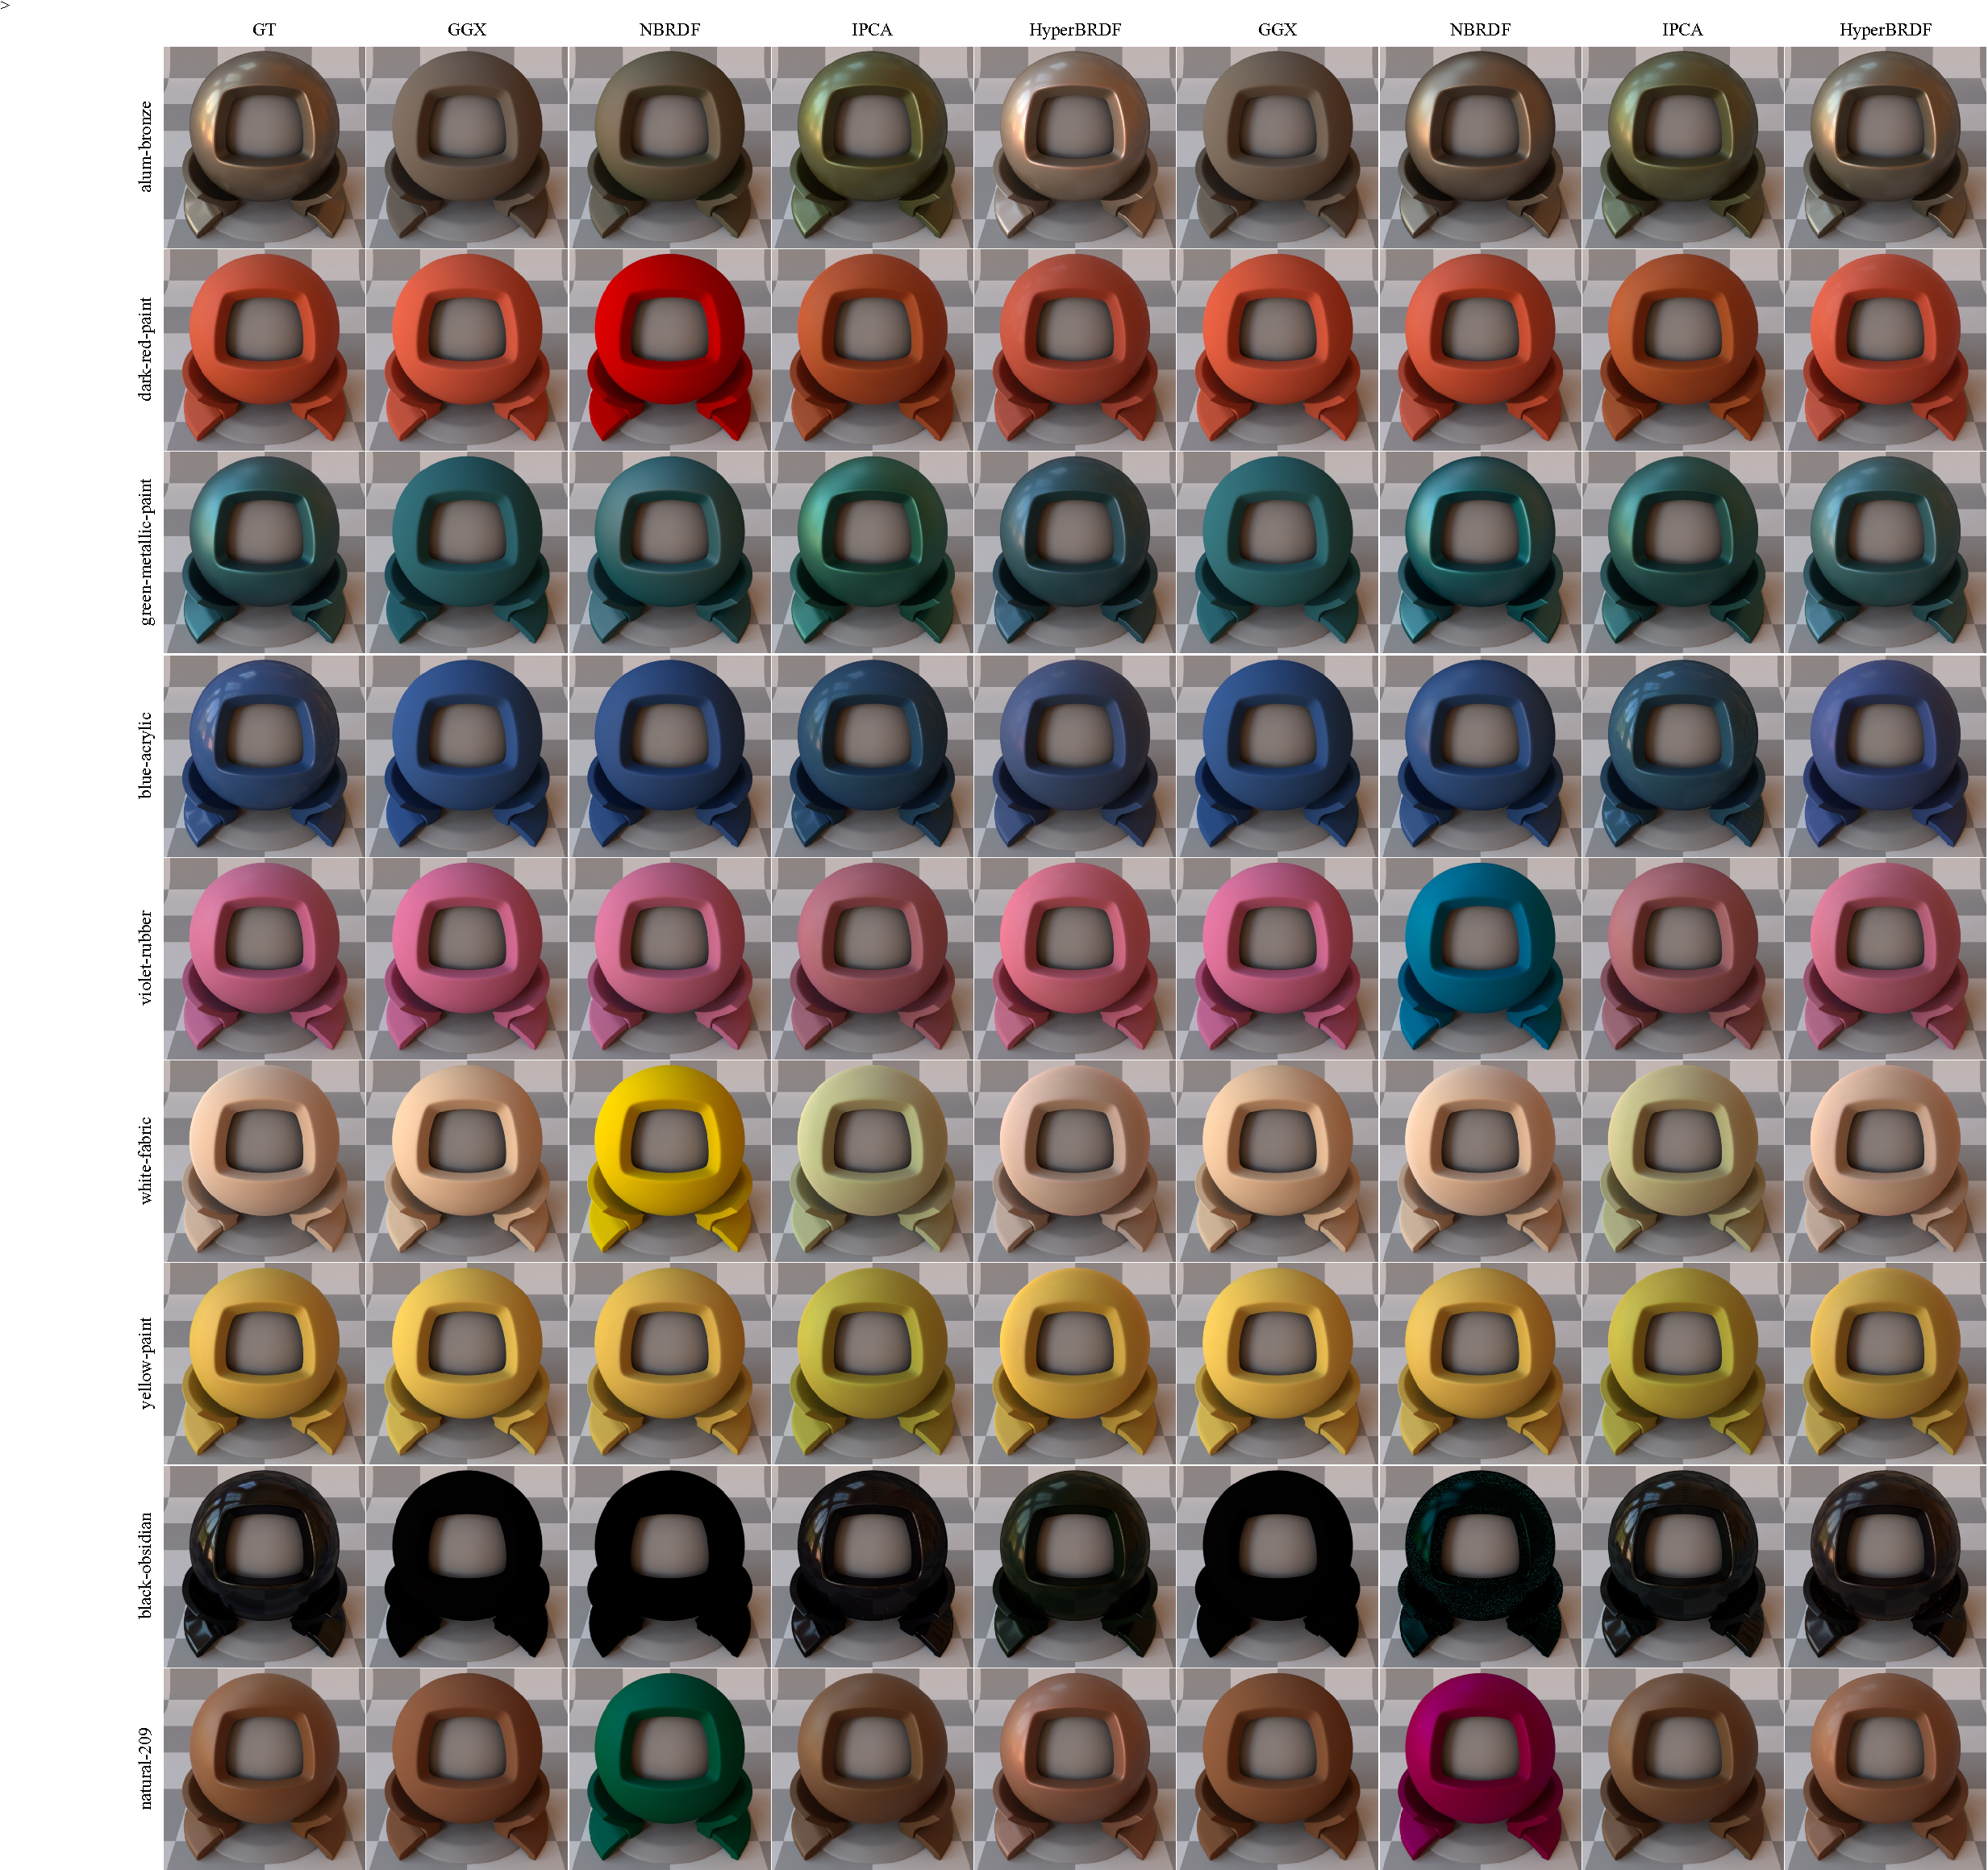
\includegraphics[width=0.9\linewidth]{Chapters/hyperbrdf-figs/qual_comp_ggx_2.pdf}}
\\
\hspace{1.9cm}{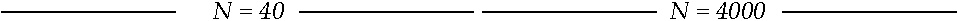
\includegraphics[width=0.73\linewidth]{Chapters/hyperbrdf-figs/N_labels2.pdf}}
   \caption{Qualitative comparison results for reconstruction with small sample sizes. Thanks to the prior that the hypernetwork model learns for material appearance through training, it can accurately estimate the BRDFs of unseen materials and preserve the colours better than the baselines.}  

   \label{fig:imp_comp_upt}
\end{figure*}

\begin{figure*}[t]
  \centering
    {
\includegraphics[width=0.35\linewidth]{Chapters/hyperbrdf-figs/legend.png}}\\
  {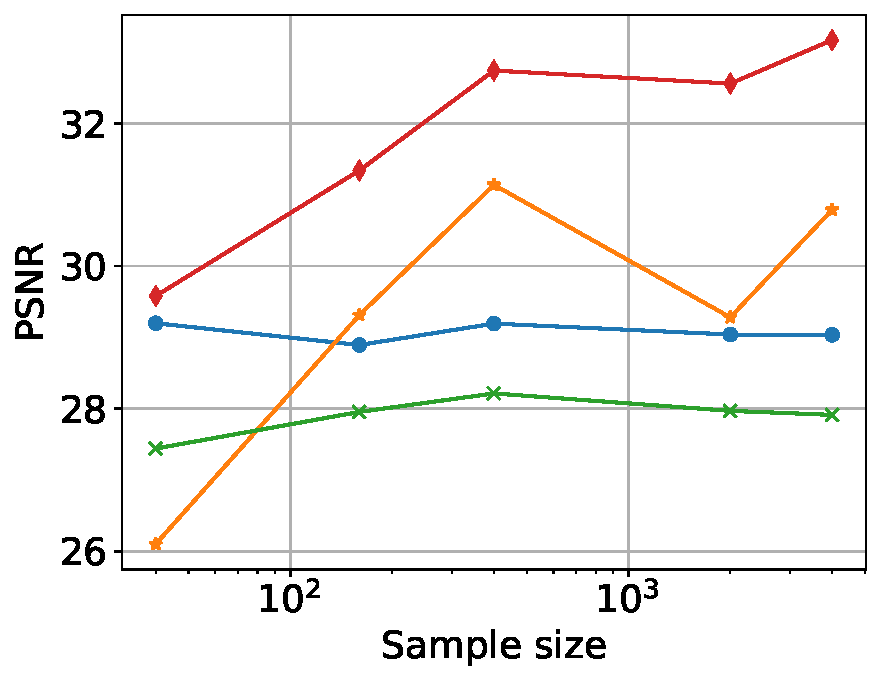
\includegraphics[width=0.32\linewidth, height=3.4cm]{Chapters/hyperbrdf-figs/PSNR_ggx.pdf}}
  {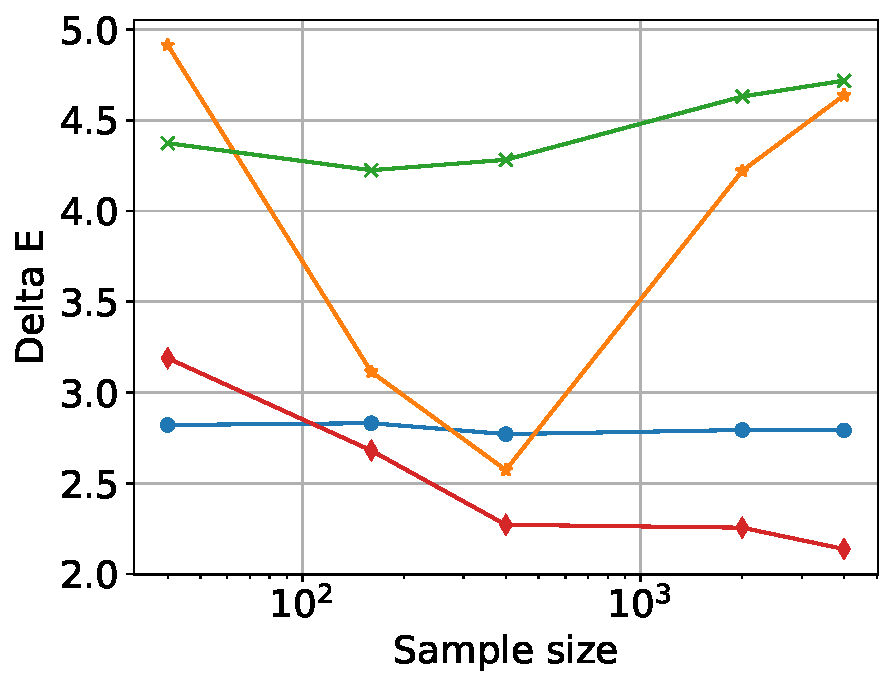
\includegraphics[width=0.32\linewidth, height=3.4cm]{Chapters/hyperbrdf-figs/DeltaE_ggx.pdf}}
  {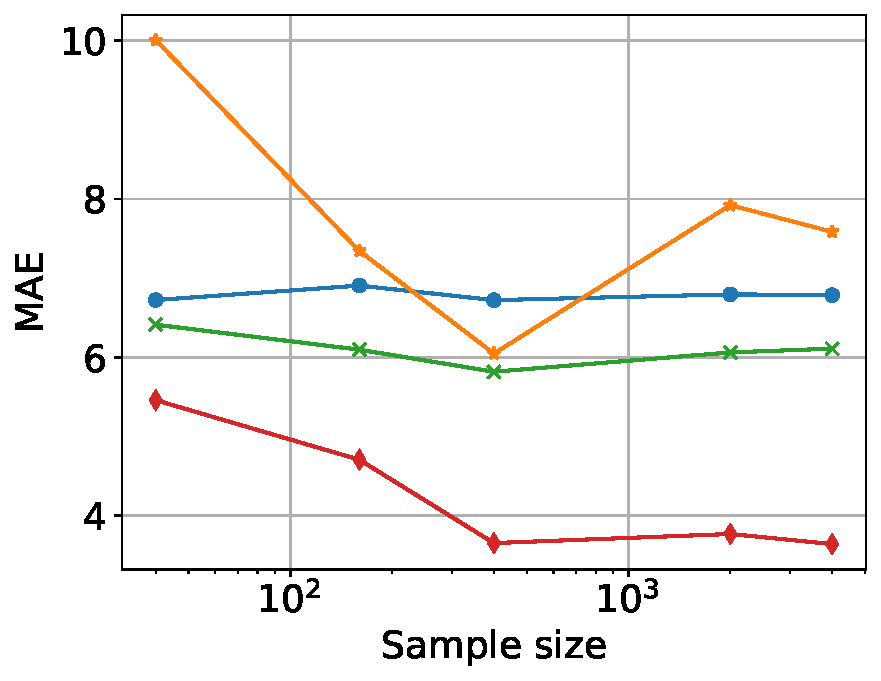
\includegraphics[width=0.32\linewidth, height=3.4cm]{Chapters/hyperbrdf-figs/MAE_ggx.pdf}}
  {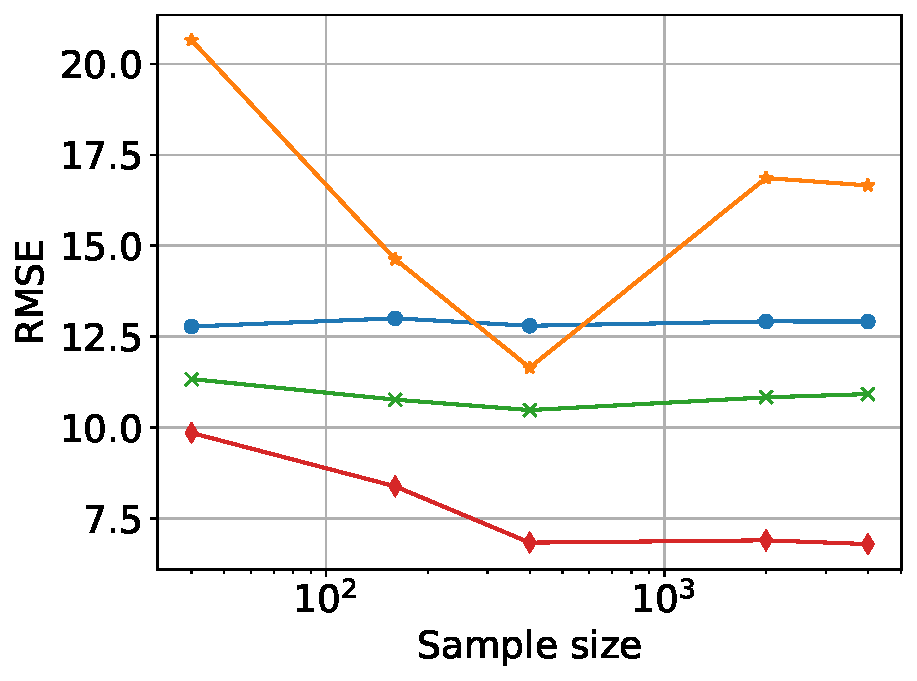
\includegraphics[width=0.32\linewidth, height=3.4cm]{Chapters/hyperbrdf-figs/RMSE_ggx.pdf}}
    {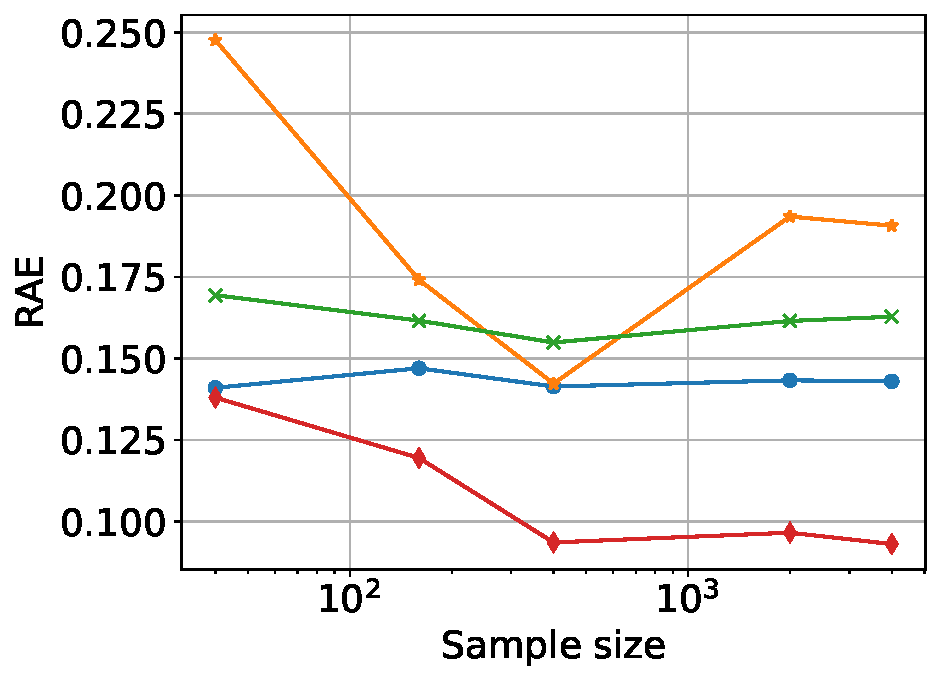
\includegraphics[width=0.32\linewidth, height=3.4cm]{Chapters/hyperbrdf-figs/RAE_ggx.pdf}}
    {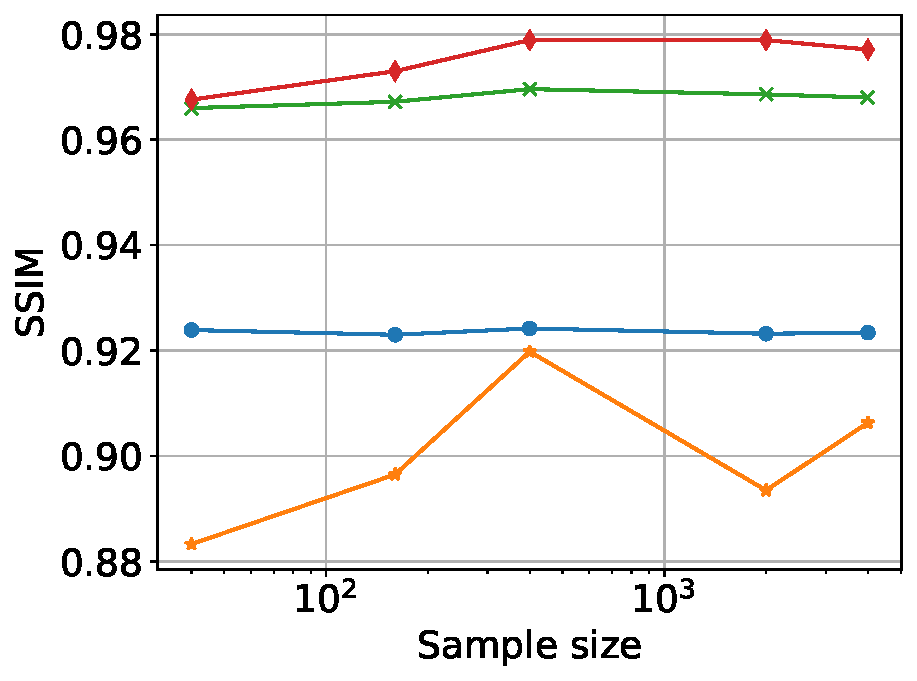
\includegraphics[width=0.32\linewidth, height=3.4cm]{Chapters/hyperbrdf-figs/SSIM_ggx.pdf}}
   \caption{Average PSNR, Delta E (CIE 2000), SSIM, MAE, RMSE, and RAE results across different sample sizes. }
   \label{fig:imp_plots}
\end{figure*}



I first compare the results with the ground truth renderings for varying sample sizes. Figure \ref{fig:imp_comp_upt} shows that the hypernetwork can still reconstruct test materials even with $N = 40$ samples. However, as I reduce the sample number to 10, the reconstruction quality highly decreases. 

During inference time, hypernetwork fits the samples to a BRDF. Even with a few samples, it can still accurately reconstruct test materials. Its success comes from the fact that it learns a prior for material appearance through training with a dataset of multiple materials. Therefore, I validate this generalizable approach by comparing the hypernetwork with an analytic model, GGX  \cite{walter2007microfacet}, NBRDF \cite{sztrajman2021neural} and PCA with Log Relative Mapping (IPCA) \cite{nielsen2015optimal}.

Sparse GGX results are obtained by fitting to the sparse number of measured BRDF samples using a non-linear optimisation (L-BFGS-B method) with Log $l_1$ loss (same loss used in NBRDF). For the results with all samples, I used the dj\_brdf mitsuba plug-in \cite{dupuy2015photorealistic}. NBRDF \cite{sztrajman2021neural} is designed to implicitly represent an individual BRDF. It can reconstruct materials with very high accuracy (Structural Similarity Index of around 0.995) when the sample size is high. It first trains the network on a material and then estimates the BRDF values of the same material. For a fair comparison, I first fit an NBRDF model to a material BRDF with the query sample size, then estimate the function with the same sample size. 

I also compare the results with a PCA-based strategy (IPCA). To represent the BRDF data, PCA-based methods  \cite{matusik2003data, ngan2006image} construct a matrix ${A} \in \mathbb{R}^{m \times n}$, where n = 180 × 90 × 90 × 3 = $4\,374\,000$ is the feature number, m = 80 is sample number. The matrix is later decomposed into its principal components via Singular Value Decomposition. PCA itself struggles with the decomposition of high dynamic range data. Therefore, the Log Relative Mapping (IPCA) is proposed~\cite{nielsen2015optimal}, which is defined in the pre-processing step (Section \ref{sec:pre-proc}). This improves the reconstruction quality, offering competitive reconstructions against HyperBRDF as shown in Figure \ref{fig:imp_comp_upt}.

For all methods including HyperBRDF, samples are drawn from a uniform distribution over Rusinkiewicz coordinates. For IPCA results, I split train and test dataset in the same way as HyperBRDF, i.e., 80 MERL materials for train and 20 for test, and use all available samples for learning the principal components. To reconstruct the test materials from sparse samples, I first run a least-squared-error optimization and predict the weights of the material for the corresponding principal components. To decide the number of components, I ran an additional ablation study, where 
I computed the average mean squared error over the test dataset for the reconstruction from sparse samples ($N = 40$). We observed that ($N_{PC} = 8$) gives the minimum error on the test dataset. Hence, I choose the number of principal components as $N_{PC} = 8$ and keep it same for sparse sampling results.

 
I keep the range for sparse sample numbers between $N = 40$ and $N = 4000$. Figure \ref{fig:imp_comp_upt} shows the rendering results for the minimum and maximum number of this range. Compared to GGX, IPCA and NBRDF, the hypernetwork can capture the appearances more precisely. Although this approach has difficulty estimating specular components (last two rows in Figure~\ref{fig:imp_comp_upt}), overall it offers reconstructions with much higher accuracy. 

I observe that the diffuse colours of some reconstructed materials by NBRDF can be completely off (natural-209, teflon) due to function fitting with sparse samples. Hypernetwork, on the other hand, can preserve diffuse colours better thanks to the prior it learns through training.


\subsubsection{Quantitative evaluation}

I compare the proposed method quantitatively with the aforementioned techniques in multiple image-based error metrics through rendering results. The metrics include peak signal-to-noise ratio (PSNR), Delta E (CIE 2000), structural similarity index (SSIM), mean absolute error (MAE), root mean square error (RMSE), and relative absolute error (RAE). I take the average over the test dataset for each metric. I plot the metric results across five different sample sizes (40, 160, 400, 2000, 4000). Since I optimize IPCA on the test dataset for the $N = 40$ case, it offers more competitive results. Nevertheless, HyperBRDF can reconstruct the BRDFs of unseen materials more precisely. Figure \ref{fig:imp_plots} shows that across all sample sizes, the hypernetwork attains superior performance in terms of PSNR, Delta E (CIE 2000) and SSIM. 

Additionally, Table \ref{table: ours_diff_samples} shows that expanding the training set, even with materials captured from a different point-based setup, helps improve the performance of the hypernetwork. Also, note that compared to MERL materials, the colours of RGL materials are more saturated, which could explain a slight increase in Delta E.


 \begin{table*}[ht]
    \centering
    \caption{Hypernetwork sparse reconstruction - Average metric results across varying sample sizes ($N$) over the test set. We highlight \colorbox{blue!25}{best} and \colorbox{orange!25}{second best} results.}
    
    {\begin{tabular}{l@{\hskip 0.4in}c@{\hskip 0.2in}c@{\hskip 0.2in}c@{\hskip 0.1in}|@{\hskip 0.1in}c@{\hskip 0.2in}c@{\hskip 0.2in}c}\toprule
    

& \multicolumn{3}{c}{MERL} & \multicolumn{3}{c}{MERL + RGL}
\\\cmidrule(lr){2-4}\cmidrule(lr){5-7}
% \toprule
  $N$ & PSNR\textuparrow & Delta E\textdownarrow & SSIM\textuparrow & PSNR\textuparrow & Delta E\textdownarrow & SSIM\textuparrow \\

 \toprule

$40$ & 29.581 & 3.189 & 0.968 & 30.018 & 3.112 & 0.963\\
$160$ & 31.341 & 2.681 & 0.973 & 31.929 & 2.454 & 0.962\\
$400$ & 32.743 & 2.272 & \cellcolor{blue!25} 0.979 & 33.855 & 2.432 & 0.977\\
$2000$ & \cellcolor{blue!25} 34.527 & \cellcolor{orange!25}2.256 & \cellcolor{blue!25} 0.979 & \cellcolor{blue!25} 34.527 & \cellcolor{orange!25} 2.243 & \cellcolor{blue!25} 0.983\\
$4000$ & \cellcolor{orange!25} 33.170 &  \cellcolor{blue!25} 2.138 & \cellcolor{orange!25} 0.977 & \cellcolor{orange!25} 34.355 & \cellcolor{blue!25} 2.166 & \cellcolor{orange!25} 0.982\\

\bottomrule
    \end{tabular}\par}
    \label{table: ours_diff_samples}
\end{table*}

\paragraph{Sparse and full reconstruction results:}

\begin{table*}[ht]
    \centering
    \caption{Hypernetwork - Average metric results across varying sample sizes ($N$) over the test set (Sparse and full reconstruction of unseen materials).}

    \resizebox{0.75\linewidth}{!}{%
    {\begin{tabular}{l@{\hskip 0.2in}c@{\hskip 0.2in}c@{\hskip 0.2in}c@{\hskip 0.2in}c@{\hskip 0.2in}c@{\hskip 0.2in}c}\toprule

 Metrics/$N$ & $8$ & $40$ & $4000$ & $40\,000$ & $640\,000$ & $1\,458\,000$\\
 \toprule
PSNR\textuparrow & 23.090 & 29.822 & 33.170 & 33.019 & \cellcolor{blue!25}33.166 & \cellcolor{orange!25} 33.128 \\
Delta E\textdownarrow & 5.948 & 3.086 & 2.138 & \cellcolor{orange!25} 2.118 & \cellcolor{blue!25}2.117 & 2.181 \\
SSIM\textuparrow & 0.927 & 0.969 & 0.977 & \cellcolor{blue!25} 0.979 & \cellcolor{blue!25} 0.979 & \cellcolor{orange!25}0.978 \\
MAE\textdownarrow & 13.167 & 5.306 & 3.642 & \cellcolor{orange!25} 3.568 & \cellcolor{blue!25}3.492 & 3.574 \\
RMSE\textdownarrow & 22.293 & 9.601 & 6.791 & \cellcolor{orange!25} 6.618 & \cellcolor{blue!25}6.507 & 6.740 \\
RAE\textdownarrow & 0.339 & 0.134 & 0.093 & \cellcolor{orange!25} 0.091 & \cellcolor{blue!25}0.089 & \cellcolor{orange!25} 0.091 \\
\bottomrule
    \end{tabular}\par}}
    \label{table: ours_large_samples}
\end{table*}


\subsubsection{Comparison with casual capture setups}
Casual BRDF estimation methods reconstruct BRDFs from a captured material image; hence, they struggle with disentangling the material from unknown illumination, often requiring a data-driven prior. As a result, most recent papers make simplifying assumptions about the material, fitting to a Phong or an analytic model. Even though iBRDF \cite{chen2021invertible} explored fitting to real-world reflectance measurements, HyperBRDF still overwhelmingly outperform their reconstruction quality with only 160 samples and above. When iBRDF is run with the same rendering setup on the same test dataset, we observe that even HyperBRDF's $N=160$ case overall offers more accurate results. Thus, casual capture remains highly impractical for professional applications mentioned earlier. Also, note that iBRDF trains their model with ground-truth measured BRDF values, and hence their requirements for supervision are no less than HyperBRDF. 


%In casual BRDF estimation, the main bottleneck lies in decoupling unknown illumination from the material, often necessitating a data-driven prior, thus is not our main focus. Consequently, most recent papers resort to assuming a Phong or analytic model for simple materials. Although iBRDF \cite{chen2021invertible} relaxed this constraint, we significantly outperform their reconstruction quality with only 160 samples and above. We ran iBRDF with the same rendering setup on our test dataset and observe that even our $N=160$ case overall offers more accurate results. Thus, casual capture remains highly impractical for professional applications mentioned earlier. We also highlight that iBRDF relies on ground-truth measured BRDF values for training, and hence requires no less supervision than ours. 

\begin{table}[ht]
    \centering
    \caption{Comparison with iBRDF \cite{chen2021invertible}  - Average metric results over the renderings of the entire MERL dataset. We highlight \colorbox{blue!25}{best} and \colorbox{orange!25}{second best} results.}

    {%
    {\begin{tabular}{l@{\hskip 0.5in}c@{\hskip 0.3in}c@{\hskip 0.3in}c}\toprule


  &  PSNR \textuparrow & Delta E \textdownarrow & SSIM \textuparrow \\
 \toprule
 HyperBRDF ($N = 400$) & \cellcolor{blue!25} 32.74  & \cellcolor{blue!25}  0.979  & \cellcolor{blue!25} 2.272\\
 iBRDF (Best) \cite{} & \cellcolor{orange!25}  31.46 &  0.954 & 2.879\\
 HyperBRDF ($N = 160$) & 31.34  & \cellcolor{orange!25}  0.973  & \cellcolor{orange!25} 2.681\\

\bottomrule
    \end{tabular}\par}}
    \label{table: oursvsibrdf}
\end{table}


\subsection{Compression}\label{sec:compression}
The high capacity of the hypernetwork also allows the compression of the densely sampled BRDF data into low-dimensional latent representations. The hypernetwork can process highly compact BRDF embeddings, and once decoded, reconstructs the BRDF data precisely. I compare HyperBRDF with Neural Processes (NPs) \cite{zheng2021compact}, the state-of-the-art BRDF compression method, and show that the hypernetwork model overall performs better in all three metrics. 


To compare this method with NPs, I overfit HyperBRDF to the mixed dataset of MERL and isotropic RGL materials, consisting of 151 materials in total. Since the latent dimension of NPs is 7D, I also train the hypernetwork with 7D latent space. It is worth mentioning that NPs cause invalid sample values in certain MERL materials, blacking some parts of the renderings. In contrast, this method consistently decompresses materials with high reconstruction accuracy; see Table \ref{table: oursvsnps}. Rendering results can be found in Appendix.

\begin{table}[ht]
    \centering
    \caption{Compression - Average metric results over the renderings of the entire MERL dataset. We highlight \colorbox{blue!25}{best} and \colorbox{orange!25}{second best} results.}

    {%
    {\begin{tabular}{l@{\hskip 0.5in}c@{\hskip 0.3in}c@{\hskip 0.3in}c}\toprule


  &  PSNR \textuparrow & Delta E \textdownarrow & SSIM \textuparrow \\
 \toprule
 HyperBRDF (40D) & \cellcolor{blue!25} 47.682 & \cellcolor{blue!25} 0.567 & \cellcolor{blue!25} 0.994\\
 HyperBRDF (7D) & \cellcolor{orange!25} 47.492 & \cellcolor{orange!25} 0.574 & \cellcolor{blue!25} 0.994\\
 NPs & 46.125 & 2.424 & 0.935\\
 IPCA & 29.892 & 3.315 & 0.979\\

\bottomrule
    \end{tabular}\par}}
    \label{table: oursvsnps}
\end{table}


\begin{figure*}[ht]
  \centering
  {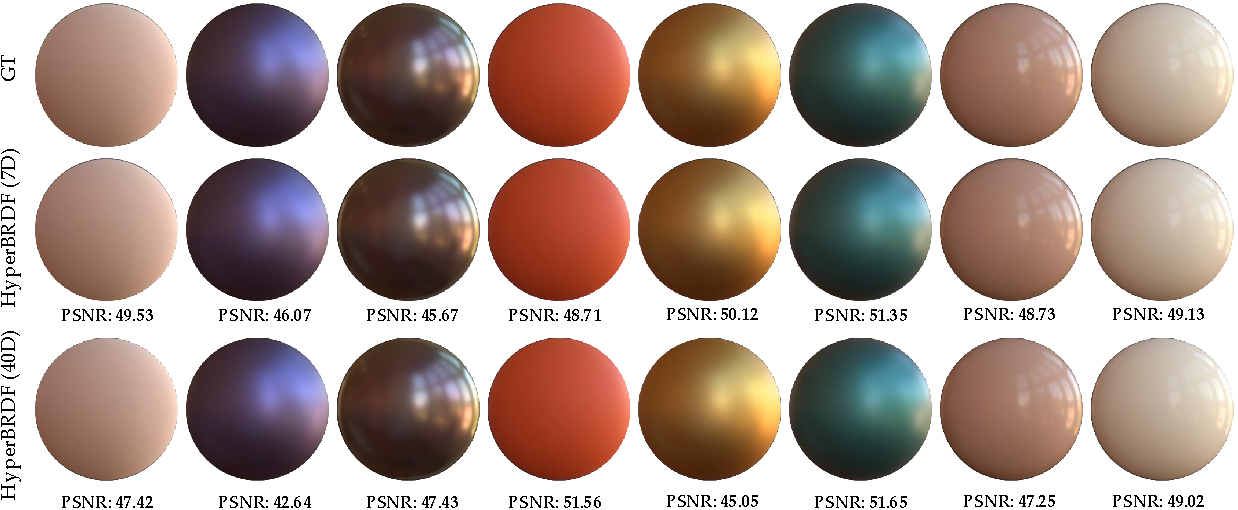
\includegraphics[width=\linewidth]{Chapters/hyperbrdf-figs/compression_comp1.pdf}}
   \caption{Reconstruction results for BRDF compression (GT: ground truths).}
   \label{fig:comp-fig}
\end{figure*}


\subsection{BRDF editing}\label{sec:brdf-editing}

Compared to analytic BRDFs that have a fixed number of parameters to tweak, editing measured BRDFs is rather a nontrivial task due to irregular data structure. On the other hand, the hypernetwork is capable of BRDF editing thanks to its representation of materials in a low-dimensional space. We can easily reconstruct various appearances by linearly interpolating between the embeddings of two different materials. Figure \ref{fig:interpolation} shows newly-reconstructed materials through linear interpolation between two different embeddings from the reconstructed MERL materials. 


\begin{figure*}[ht]
  \centering
  % \fbox{\rule{0pt}{2in} \rule{0.9\linewidth}{0pt}}
   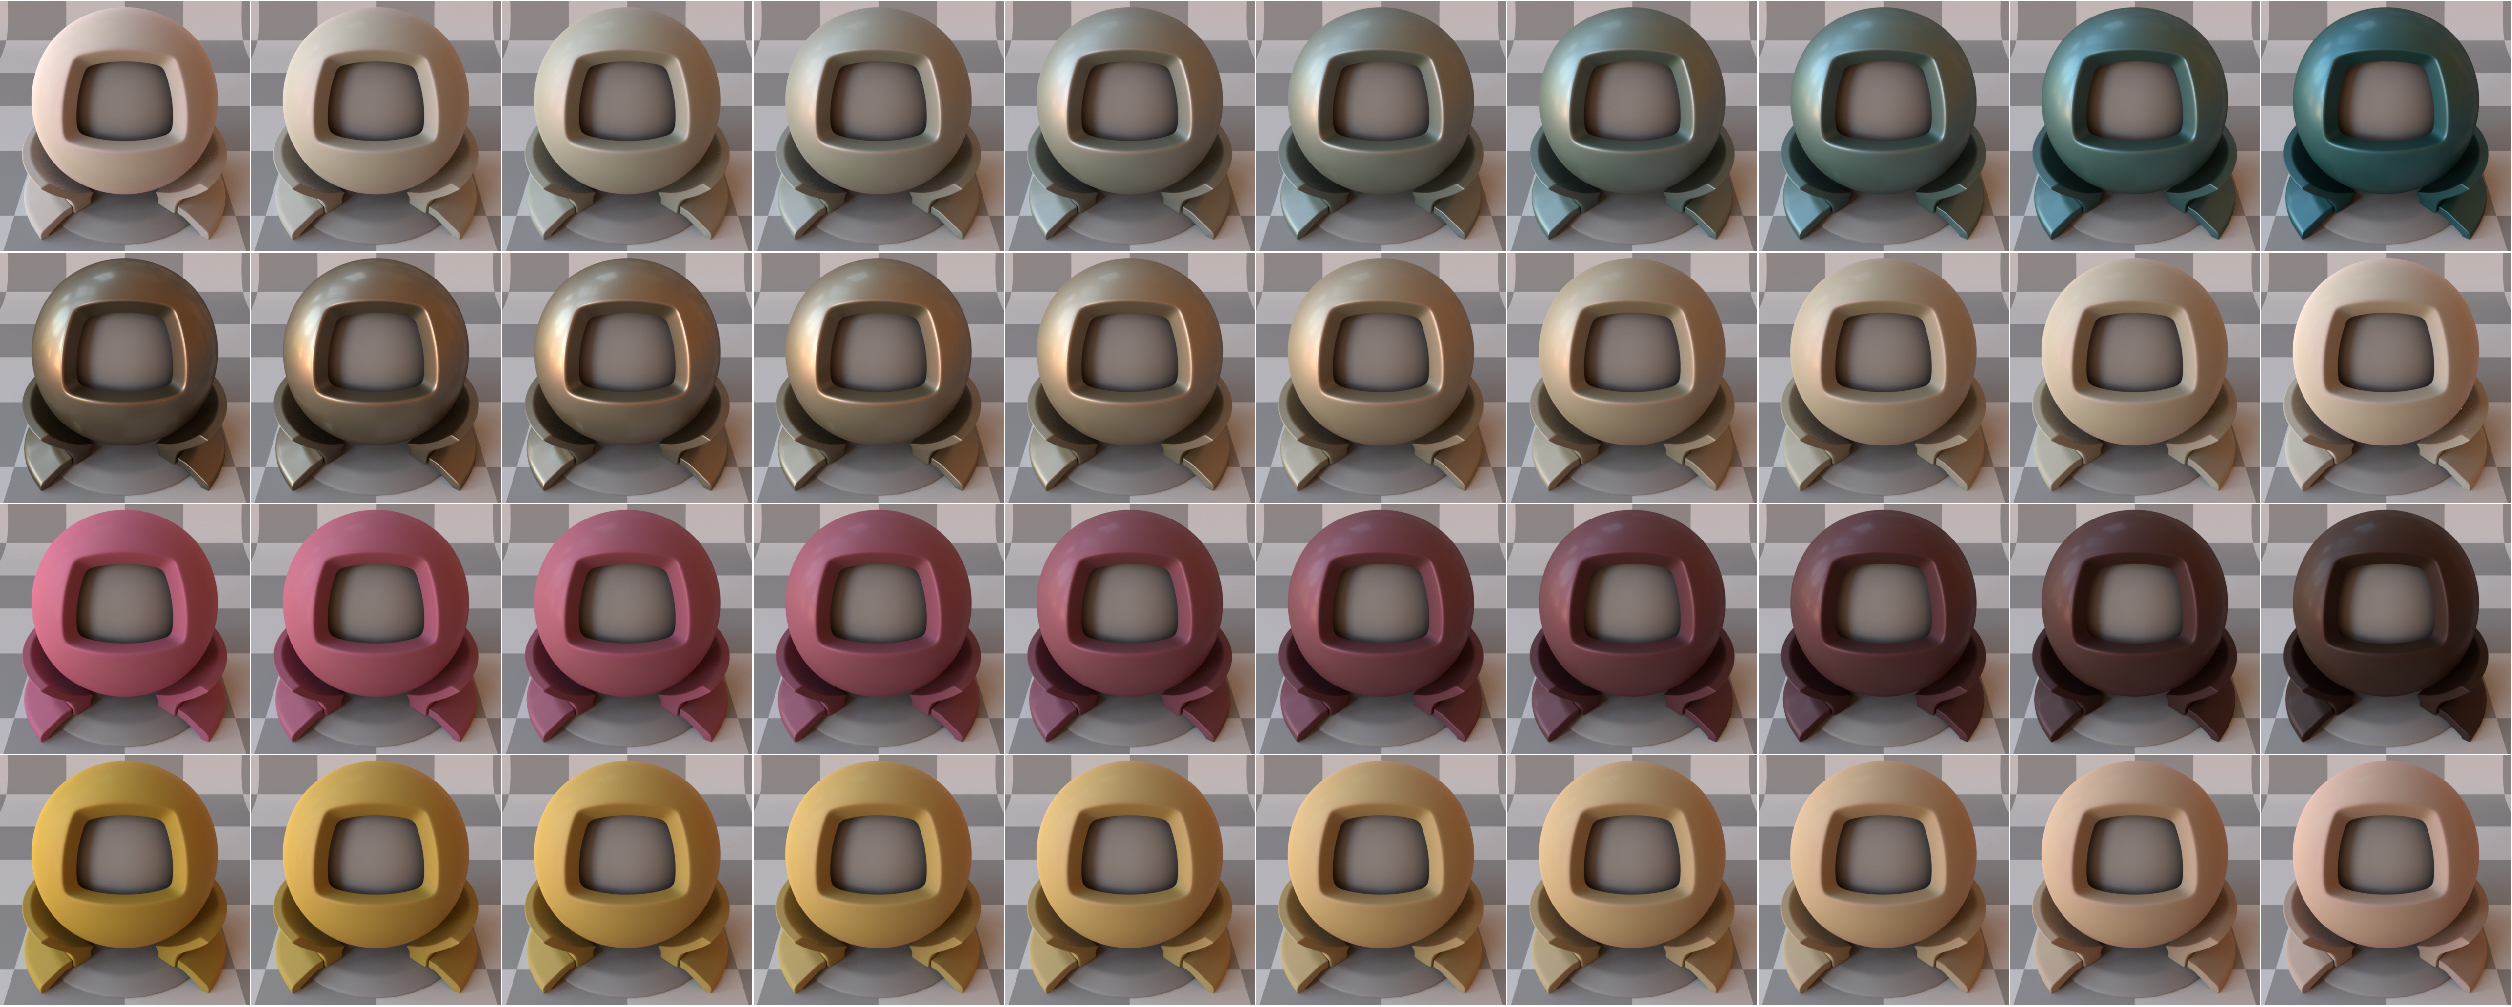
\includegraphics[width=\linewidth]{Chapters/hyperbrdf-figs/interpolation_extended.pdf}

   \caption{BRDF editing through linear interpolation between the embeddings of two materials.}
   \label{fig:interpolation}
\end{figure*}

\subsection{Ablation studies}\label{sec:abl}
\subsubsection{Latent dimension}
I experimented with the dimension size of the latent representations $Z$ on the test dataset for the reconstruction with all available samples and observed that 40-dimensional embeddings give the minimum average mean squared error (See the first row of Table \ref{table: z_abl}). Therefore, I chose the latent space size to be 40. However, I also observed that these can change with the number of sparse samples. For consistency, I kept it same for all the reconstruction results. 

\subsubsection{Log relative mapping (LRM)}\label{sec:lrm}
I apply Log Relative Mapping (LRM) \cite{nielsen2015optimal} to the BRDF data before feeding it the hypernetwork, as described in Section \ref{sec:pre-proc}. I illustrate that LRM improves the reconstruction quality for both PCA and hypernetwork results in Table \ref{table: comparison results} and Figure \ref{fig:qual_comp}. Please note that IPCA is the mapping-applied version of PCA, and "HyperBRDF (No LRM)" refers to HyperBRDF results without LRM.


\subsubsection{Cosine weighting}
Similar to \cite{ngan2005experimental}, I also weigh the BRDFs with a cosine term based on the assumption of uniform incoming radiance and observed that it offers higher accuracy:

\begin{table}[ht]
    \centering
    \caption{Average metric results over the renderings of the test set (20 MERL materials).}

    {\begin{tabular}{l@{\hskip 0.3in}c@{\hskip 0.3in}c@{\hskip 0.3in}c}\toprule
    % \resizebox{0.5\linewidth}{!}{%
    % {\begin{tabular}{ccc}\toprule

 &  No Cosine &  Cosine\\
 \toprule
 PSNR\textuparrow & 33.077 & \cellcolor{blue!25} 33.166 \\
Delta E\textdownarrow & 2.233 & \cellcolor{blue!25} 2.117 \\
SSIM\textuparrow & 0.974 & \cellcolor{blue!25} 0.979 \\
MAE\textdownarrow & 3.908 & \cellcolor{blue!25} 3.492 \\
RMSE\textdownarrow & 7.370 & \cellcolor{blue!25} 6.507 \\
RAE\textdownarrow & 0.098 & \cellcolor{blue!25} 0.089 \\
\bottomrule
    \end{tabular}\par}
    \label{table: cos_abl}
\end{table}

\subsubsection{Principal component analysis (PCA)}
In Section \ref{sec:qual_comp}, I briefly discussed the ablation study I ran to choose the number of principal components for the best-performing IPCA results. Here, I elaborate on the effect of the number of principal components on the performance of IPCA. 


\paragraph{Number of Principal Components:}
I analyzed the optimal number of principal components by initially choosing the same numbers as we did for the ablation study of the latent dimension. Looking at Table \ref{table: z_abl}, I observe that $N_{PC}$ gives the minimum error for sparse cases, where the number of samples $N$ is 40. I further validated the choice $N_{PC} = 8$ by running IPCA with the number of principal components ranging from 1 to 16 with an incremental change of 1. Figure \ref{fig:ipca_opt} illustrates that $N_{PC} = 8$ still gives the minimum mean squared error (MSE) averaged over the test set.


\begin{figure}[ht]
  \centering

  {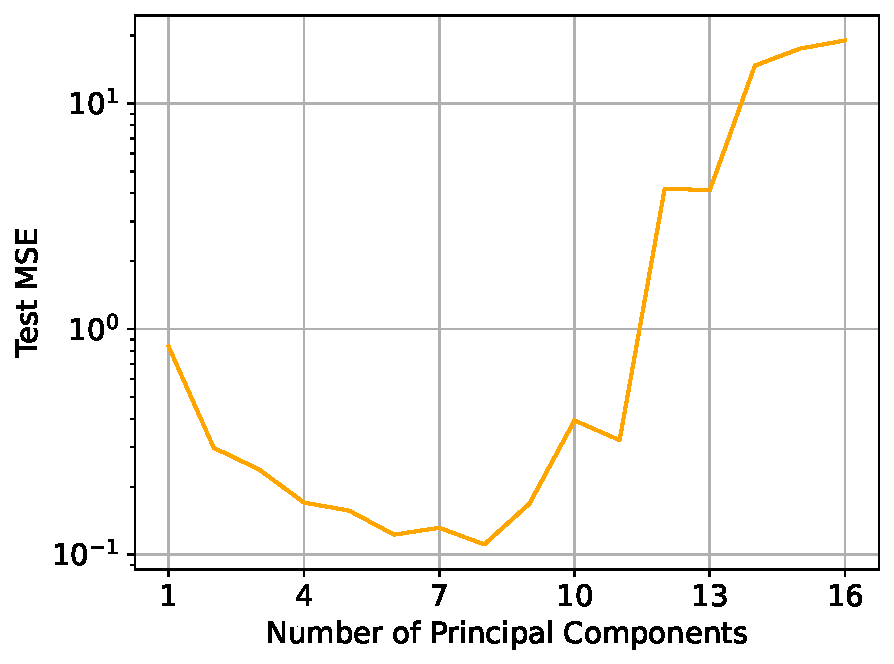
\includegraphics[width=0.6\linewidth]{Chapters/hyperbrdf-figs/ipca_opt_q_40_cropped.pdf}}
   \caption{IPCA optimization for the number of principal components.}
   \label{fig:ipca_opt}
\end{figure}

\begin{table*}[ht]
    \centering
    \caption{Average mean squared errors for varying latent space dimensions (first row) and number of principal components (second row)}

    \resizebox{0.9\linewidth}{!}{%
    {\begin{tabular}{l@{\hskip 0.1in}c@{\hskip 0.1in}c@{\hskip 0.1in}c@{\hskip 0.1in}c@{\hskip 0.1in}c@{\hskip 0.1in}c@{\hskip 0.1in}c@{\hskip 0.1in}c}\toprule

 Methods/Dimension & 8 & 20 & 30 & 40 & 50 & 60 & 70 & 80\\
 \toprule
  HyperBRDF & 0.073 & \cellcolor{orange!25} 0.046 & 0.062 & \cellcolor{blue!25} 0.045 & 0.051 & 0.053 & 0.049 & \cellcolor{orange!25} 0.046\\
 IPCA & \cellcolor{blue!25} 0.131 & 0.278 & 12.288 & \cellcolor{orange!25} 0.507 & 0.878 & 0.883 & 0.965 & 1.124\\
 
\bottomrule
    \end{tabular}\par}}
    \label{table: z_abl}
\end{table*}


\subsection{Scene renderings}
I also rendered multiple scenes \cite{resources16} using HyperBRDF's reconstructed materials, including sparse reconstruction, compression and interpolation. The details about the objects covered with HyperBRDF's reconstructed materials are as follows (Figure \ref{fig:scene-render}): \textbf{\textit{teapot:}} steel. \textbf{\textit{dragons:}} interpolation of delrin and green-metallic-paint, white marble (dragon paint), silver-metallic-paint3 (ground), dark-red-paint (cloth). \textbf{\textit{cars:}} chrome steel, gold metallic paint3, specular-red-phenolic (car paint), exterior car parts (aluminium), inner wheel (alumina-oxide). \textbf{\textit{kitchen:}} cupboards (natural-209), utensils (chrome), handles, pot, microwave and cooker (two-layer-silver), extractor hood (aluminium), pot and kettle handles (black-obsidian), kettle paint (dark-red-paint), tea towel and cushions (yellow-paint), radio and lamp (polyethylene). \textbf{\textit{living room:}} sofa, coffee table, side tables, wall book shelf (pure-rubber), cushions (green-metallic-paint), twigs (natural-209), legs (dark-specular-fabric).
\textbf{\textit{sofas:}} violet rubber and green latex (sofa cover). 

\begin{figure}[ht]
  \centering
  {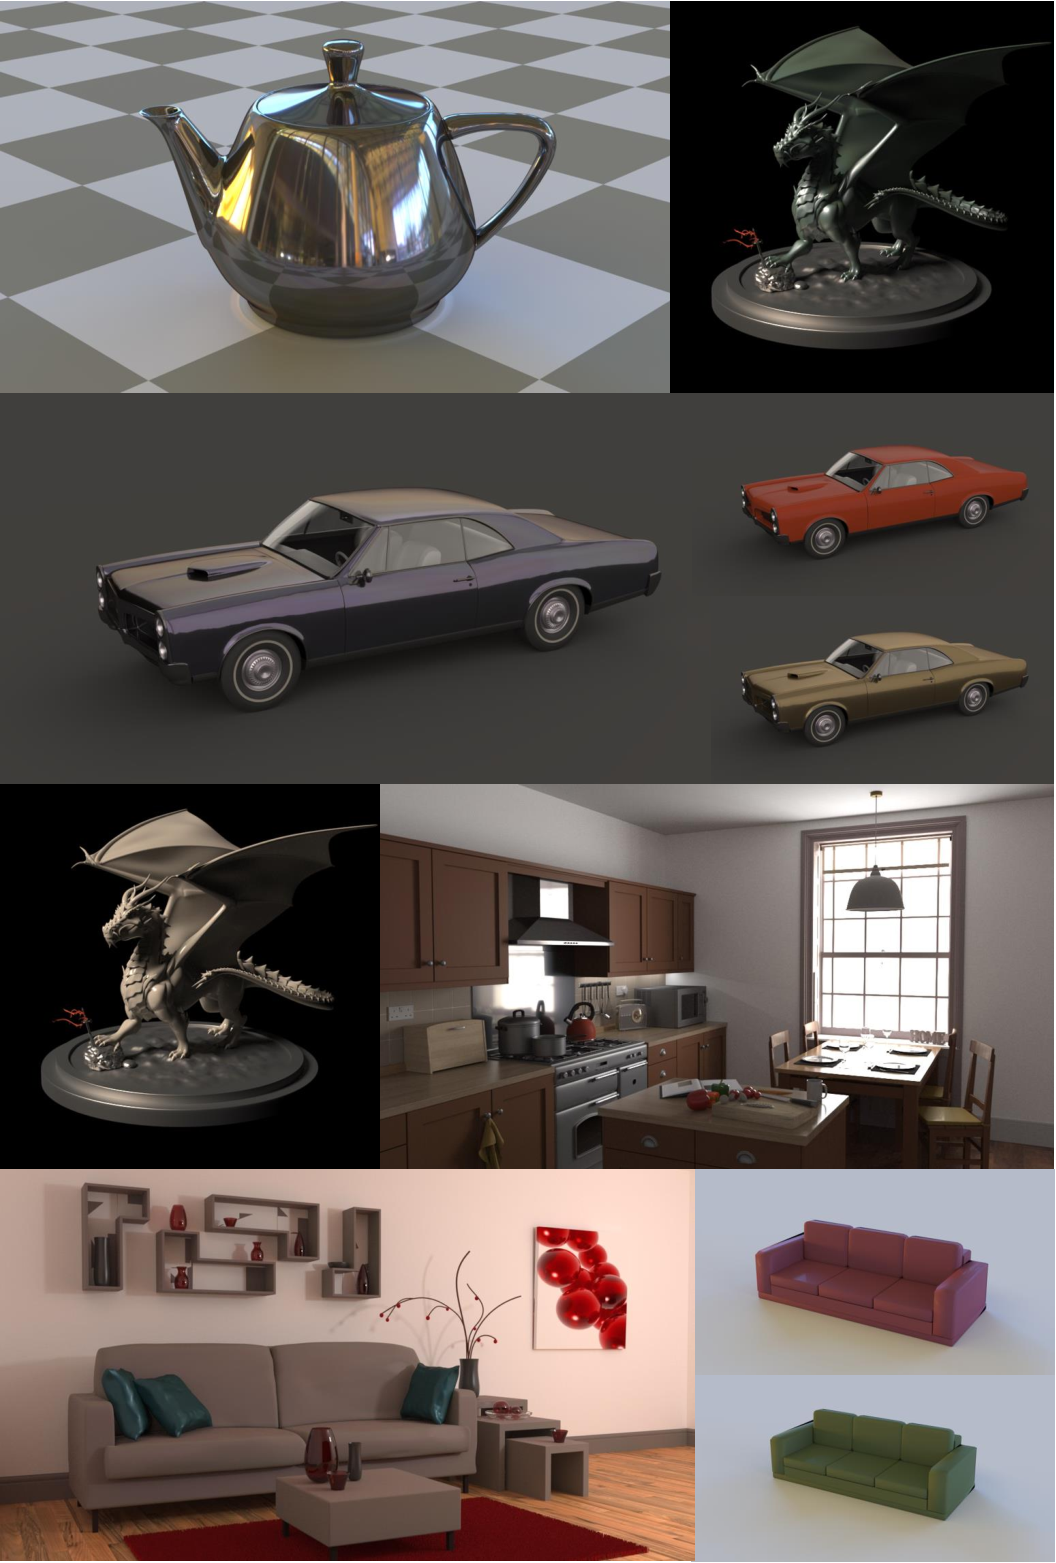
\includegraphics[width=\linewidth]{Chapters/hyperbrdf-figs/SceneRenderings1.pdf}}
   \caption{Scene renderings with materials reconstructed by HyperBRDF.}
   \label{fig:scene-render}
\end{figure}

\subsection{Limitations and future work}\label{sec:limits}
\paragraph{Specular components:} HyperBRDF struggles with the estimation of specular components as shown in Figure~\ref{fig:imp_comp_upt} (last two rows). It is likely because of the high gap between the values of diffuse that are close to zero and the values of specular components that are arbitrarily high. A separate estimation pipeline for each component within the network can help improve the results.


\paragraph{BRDF editing:} The BRDF editing approach is rather non-intuitive with an interpolation approach. Finding a map between the embeddings and certain attributes of the materials, such as diffuse/specular colours or haziness, can lead to more interactive BRDF editing. I plan to map the latent space to material parameter space so that users can easily edit materials through more interpretable parameters.

\paragraph{SVBRDF representations:} In this work, I focused on the task of generalizable neural representations for spatially uniform BRDFs. As the future work, I plan to extend HyperBRDF to SVBRDF representations.
